% !TeX root = manifold.tex
% author: buwailee@nmhs
\chapter{Calculus}
\section{Foundation}

\para 一个局部$n$维欧几里得空间是一个Hausdorff空间$M$满足,对每一个点$p\in M$,存在一个$p$的邻域$U\osub M$和一个同胚$\varphi:U\to V$,其中$V$是一个$\rr^n$中的开集。这个同胚有时候被称为一个坐标、坐标映射等,而资料$(U,\varphi)$被称为一个\idx{坐标卡}。坐标$\varphi$经常写成分量形式,$\varphi=(x^1,\cdots,x^n)$,其中$x^i:U\to \rr$.

一个局部$n$维欧几里得空间是局部紧的,这是因为他局部同胚于欧式空间, 而欧式空间是局部紧的。

\para 局部欧几里得空间$M$上的一个光滑微分结构$\mathscr{F}$是这样一族坐标卡$(U_\alpha,\varphi_\alpha)$,满足:$\{U_\alpha\}$构成$M$的开覆盖,$\varphi_\alpha\circ\varphi^{-1}_\beta|_{U_\alpha\cap U_\beta}$是光滑映射,后者被称为坐标卡的相容性条件。此外,如果有一个坐标卡$(U,\varphi)$和每一个坐标卡都相容,那么可以推断出他在$\mathscr{F}$中,这样的微分结构被称为极大微分结构。极大微分结构当然不一定是唯一的,不过我们不担心这个,因为我们往往是固定一个微分结构来研究流形的几何,下面假设出现的微分结构总是极大的。

\para 设$(M,\mathscr{F})$和$(N,\mathscr{G})$是两个光滑流形,连续函数$f:M\to N$被称为一个\idx{光滑映射},如果$\psi\circ f\circ \varphi^{-1}$是一个光滑函数对任意的$\mathscr{F}$中的坐标卡$(U,\varphi)$和$\mathscr{G}$中的坐标卡$(V,\psi)$成立。由于欧式空间之间的光滑函数的复合依然是光滑的,所以光滑的定义是不依赖于坐标卡的选取的。

\para 这样,光滑流形就构成了一个范畴,其中态射是流形间的光滑映射。他是拓扑空间范畴的子范畴。

从此以后,我们对一个固定的流形$(M,\mathscr{F})$,常常会略去他的微分结构,只写作$M$。对于一个光滑流形$M$的非空开子集$U$,显然,他有继承自$M$的一个拓扑结构和微分结构,所以$U$也是一个光滑流形。很容易看到,$\rr^n$是一个光滑流形,按照上面的结论,我们可以得到一类光滑流形,$\rr^n$的开子集。比如把$n\times n$矩阵放入$\rr^{n^2}$内,那么行列式不为零的那些矩阵就构成一个光滑流形,记作$\mathrm{GL}(n,\rr)$,称作一般线性群。

特别地,$\rr$也是一个光滑流形。我们称光滑映射$f:M\to \rr$是一个$M$上的光滑函数。光滑函数$f$限制在$U\osub M$上也是一个光滑函数$f|_U$.

\para 设$M$是一个光滑流形,$U\osub M$上的光滑函数的集合记作$\calf(U)$,$\calf$被称为$M$上的光滑函数\idx{层}。由于可以逐点定义加法和乘法,所以$\calf(U)$拥有$\rr$-代数结构。设$p\in M$,我们定义如下等价关系:设$U$和$V$都是$p$的邻域,以及$f\in \calf(U)$和$g\in \calf(V)$,如果在一个$W\osub U\cap V$上,$f|_W=g|_W$,则$f\sim g$. 所有这样的等价类记作$\calf_p$,称为$p$处的光滑函数\idx{茎},他的代表元素可以写成$f_p=\langle U,f\rangle$,称为\idx{芽}. 显然$\calf_p$有继承自$\calf(U)$的自然的$\rr$-代数结构。上述过程也可以用colimit表示为$\calf_p=\varinjlim_{U\ni p}\calf(U)$,其中$p$的邻域以包含形成归纳系。

设$p\in M$,茎$\calf_p$是一个局部环。实际上,$\langle U,f\rangle \in \calf_p$且$f(p)= 0$的元素构成了$\calf_p$的一个理想。不在这个理想内的$\langle U,f\rangle$,由于$f(p)\neq 0$,那么适当缩小$U$到$V$,由$f$的连续性,总可以找到$V$使得$f|_V$处处不为零,这样$\langle V,1/f|_V\rangle$便是$\langle U,f\rangle$的一个逆。因此上面这个理想即$\calf_p$唯一的极大理想,我们其记作$\mm_p$。容易看到$\calf_p/\mm_p\cong \rr$,实际上,对每一个芽$f_p\in\calf_p$,都成立$f_p=f_p-f(p)+f(p)$,在$\calf_p/\mm_p$中看,他和$f(p)\in\rr$也就没区别了。

\lem 设$f:\rr^n\to \rr$光滑,则
\[
	f(x)=f(0)+\partial_if(0)x^i+\frac{1}{2}g_{ij}(x)x^ix^j,
\]
其中$g_{ij}$光滑。

\proof 利用微积分基本定理
\[
	f(x)-f(0)=\int_0^1f'(tx)\dd t=\int_0^1\partial_i f(tx)x^i\dd t=h_i(x)x^i,
\]
可以得到$h_i(0)=\partial_i f(0)$,然后再对$h_i$使用上面的步骤即可得到我们想要的表达式。\qed

\para 使用一个局部坐标$\varphi=(x^1,\cdots,x^n)$且$\varphi(p)=0$,可以将上面的引理翻译到流形上。设$f:U\to \rr$光滑,则在$p$的一个邻域$V$上对任意的$q\in V$成立
\[
	f(q)=f(p)+\frac{\partial f\circ \varphi^{-1}}{\partial x^i}(p)x^i(q)+\frac{1}{2}g_{ij}(q)x^i(q)x^j(q),
\]
其中$g_{ij}$在$V$上光滑,以后我们就将那个偏微分记作$\partial_i f(p)$.


\para 设$p\in M$,$p$处的茎为$\calf_p$,他的极大理想为$\mm_p$,此时$p$处的\idx{余切空间}被定义为自然的矢量空间$T_p^*M:=\mm_p/\mm_p^2$。余切空间的元素被称为\idx{余切矢量}。

$\mm_p/\mm_p^2$确实是一个矢量空间。首先它显然是一个$\calf_p$-模,然后任取$a\in \mm_p$,由于$a\mm_p/\mm_p^2=0$,所以$\mm_p/\mm_p^2$是一个$\calf_p/\mm_p$-模,即$\rr$-矢量空间。这样定义的余切空间,可以看到,是所有的那些一阶小量构成的集合,即其中的元素为“{微分\kaishu}”。

\para 设$p\in M$,$M$是一个$n$维流形,则$T_p^*M:=\mm_p/\mm_p^2$是$n$维的。

我们可以选取一组局部坐标来算维数,由于选取不同的局部坐标都是通过同胚联系的,所以不同的选取对维数没什么影响。由上面的引理,设$f_p\in \mm_p$,则他可以写作
\[
	f_p=\partial_i f(p)x^i_p+\frac{1}{2}g_{ij}(q)x^i_px^j_p
\]
考虑一个局部坐标$\varphi=(x^1,\cdots,x^n)$,设自然同态$\dd_p:\mm_p\to \mm_p/\mm_p^2$,很简单就可以看到$\dd_p(x^i_p)\neq 0$.实际上,如果$x^i_p\in \mm_p^2$,那么$x^i_p=rs$,其中$r$, $s\in \mm_p$,然后根据上面的引理$r=a_ix^i_p+\cdots$以及$s=b_ix^i_p+\cdots$,于是$x^i=rs=a_jb_kx^j_px^k_p+\cdots$,但显然这是不可能的。

所以,如果$f_p\in \mm_p$,则
\begin{equation}
\label{c1:e1}
	\dd_p(f_p)=\partial_i f(p)\dd_p(x^i_p).
\end{equation}
这样所有的$T_p^*M=\mm_p/\mm_p^2$中的元素都可以由$\dd_p(x^i_p)$展开,他们都是非零的,而且容易证明是线性无关的,所以这是$T_p^*M$的一组基,余切空间的维数计算完毕。

以后我们用$\dd_p(f)$乃至$\dd_pf$来记$\dd_p(f_p)$。实际上,我们可以将$\dd_p$定义在$\calf_p$上,设$a$是一个常值芽,补充定义$\dd_pa=0$,可以看到,此时式\eqref{c1:e1}依旧满足。以后我们就这样来看$\dd_p:\calf_p\to T_p^*M$,他被称为\idx{外微分}算子。

\para 此时\[\dd_p (fg)=\dd_p\bigl(\bigl(f-f(p)\bigr)\bigl(g-g(p)\bigr)+f(p)\bigl(g-g(p)\bigr)+\bigl(f-f(p)\bigr)g(p)\bigr)=f(p)\dd_pg+\dd_pf g(p).\]

\para 设$f:M\to N$是一个光滑映射,上面的光滑函数层分别为$\calf$和$\calg$。任取$\varphi\in \calg(V)$,可以通过$f^*\varphi=\varphi\circ f$定义$f^*\varphi\in \calf(f^{-1}(V))$.

下面我们考虑两个流形余切空间之间的映射。设$\langle V,\varphi\rangle\in \calg_{f(p)}$,于是$\langle f^{-1}(V),\varphi\circ f\rangle\in \calf_p$,所以$f^*$诱导了一个$\rr$-代数同态$f^*_p:\calg_{f(p)}\to \calf_p$,特别地,可以看到$f^*_p:\mm_{f(p)}\to \mm_{p}$,于是$f^*_p:\mm^2_{f(p)}\to \mm^2_{p}$.

\para 设$f:M\to N$是一个光滑映射,他诱导了一个线性映射\footnote{这里我们滥用一下记号。}$f^*_p:T_{f(p)}^*N\to T_p^*M$.

对于复合,显然$(f\circ g)^*=f^*\circ g^*$,以及在一点处,$(f\circ g)^*_p=g^*_p\circ f^*_{g(p)}$.很容易看到$\id^*_p=\id_{T_p^*M}$,所以如果$f:M\to N$是同胚,则$f_p^*:T_{f(p)}^*N\to T_p^*M$是同构。

\para \label{f*d=df*}利用复合公式,设$f:M\to N$是光滑映射,则$f^*_p\bigl(\dd_{f(p)}g\bigr)=\dd_{p}(f^*g)=\dd_p(g\circ f)$.

\para 设$p\in M$,$M$是$n$维光滑流形,则\idx{切空间}$T_pM$被定义为余切空间$T_p^*M$的对偶空间。切空间的元素被称为\idx{切矢量}。由于余切空间是有限维的,他的对偶空间也和他有着相同的维度,即$n$维。

\para 由于切空间是余切空间的对偶空间,所以他是余切空间上的线性函数构成的空间,反过来,由于是有限维的,所以可以认为对偶空间的对偶空间就是原本的空间,这就是说可以将余切空间的矢量看成切空间矢量的线性函数:设$\dd_p f\in T_p^*M$和$v\in T_pM$,定义$\dd_p f(v):=v(\dd_p f)$.

虽然上面这些个定义都很短也很清楚,不过操作上却没有那么简单。下面,我们将一个切矢量扩张到$\calf_p^*$上面去。

设$f$是在$p$附近的光滑函数,而$v\in T_pM$,可以通过$D_v(f_p):=v(f_p-f(p))$定义线性映射$i_p:v\mapsto i_p(v)=D_v\in \calf_p^*$,他是一个单射。

注意到$(fg)_p=f_pg_p$,所以
\begin{align*}
	D_v(f_pg_p)&=v(f_pg_p-f(p)g(p))\\
	&=v\bigl((f_p-f(p))(g_p-g(p))+f(p)(g_p-g(p))+(f_p-f(p))g(p)\bigr)\\
	&=f(p)D_v(g_p)+D_v(f_p)g(p),
\end{align*}
我们将满足这条性质的线性映射$D_v\in \calf_p^*$称为$p$处的导子,所有$p$处的导子构成的空间暂时记作$V_p$,而他其实和$T_pM$是同构的。

为了证明这点,任取导子$D\in V_p$,由于$D(1)=D(1\times 1)=2D(1)$,所以$D(1)=0$,继而靠着$D$的线性性,对于常值函数的芽$a$来说,$D(a)=aD(1)=0$。因为每一个$\calf_p$中的元素$f_p$都可以写成$f_p-f(p)+f(p)$的形式,所以$D(f_p)=D(f_p-f(p))$,这就是说,一个导子的性质完全由他在$\mm_p$上的值决定,这种关系是一对一的。即$\pi_p:D\mapsto D|_{\mm_p}$是一个线性同构。

同时,设$f_p$, $g_p\in \mm_p$,则$\pi_p(D)(f_pg_p)=f(p)\pi_p(D)(g_p)+g(p)\pi_p(D)(f_p)=0$,于是$\pi_p(D)(\mm_p^2)=0$,所以,$\pi_p(D)\in T_pM$,即$D|_{\mm_p}$是一个切矢量,因此导子$D$完全由一个切矢量$D|_{\mm_p}=\pi_p(D)$决定。这样,$i_p:T_pM\to V_p$也是一个满射,所以他是一个同构。当然我们也可以直接计算验证$\pi_p\circ i_p=\id_{T_pM}$以及$i_p\circ \pi_p=\id_{V_p}$。

因为有这个同构,所以以后我们用$T_pM$来标记导子构成的矢量空间,一个导子才是一个切矢量。这样的好处是,我们在具体计算的时候,可以直接在$\calf_p$上进行而非$\mm_p$上,特别地,现在对于一个切向量$v$来说,成立$\dd_pf(v)=v(f_p)$,这是因为对一个导子$v$来说$v(f_p)=v(\dd_pf)$.

\para 设$f:M\to N$是一个光滑映射,定义它在$p\in M$处的导数为$T_pf=f_{*p}:T_pM\to T_{f(p)}N$使得对任意的$v\in T_p M$和任意的$g_{f(p)}\in \mm_{f(p)}$成立$(f_{*p}v)(g_{f(p)})=v(f_p^*g_{f(p)})$.

为以后的处理方便,不妨通过等同$\partial_i$和标准基$e_i$来等同$T_p\rr^n$和$\rr^n$。此外,通过坐标卡上的同胚$\varphi$,我们用$\partial_i$来标记$\varphi^{-1}_{*p}(e_i)$,这显然是$T_pM$处的一组基。


\para 设$f$是在$p$附近的光滑函数,任取$v\in T_pM$.因为$f_{*p}:T_pM\to T_{f(p)}\rr=\rr$,所以$f_{*p}(v)$是一个数,故而
	\[
		f_{*p}(v)=f_{*p}(v)(\id_{\rr})=v\bigl((\id_{\rr}\circ f)_p\bigr)=v(f_p)=\dd_p f(v).
	\]
	因为对所有的切矢量$v$都成立上式,所以$f_{*p}=\dd_p f$.

选定一个局部坐标,因为$\dd_p x^i(\partial_j)=\partial_jx^i(p)=\delta^i_j$,所以$\dd_p x^i$就是$\partial_i$的对偶基。下面我们来计算一个特别的例子,设$f:M\to \rr^n$是一个流形$M$上的矢量值光滑函数,则$f^i:M\to \rr$是一个光滑函数,那么$f_{*p}=\dd_pf^i e_i$,其中$e_i$是$\rr^n$的标准基。再设$f:\rr^m\to \rr^n$,则$\dd_pf^i=\partial_j f^i(p) \dd x^j=\partial_j f^i(p) e^j$.写成矩阵即
\[
	(f_{*p})^{i}_{\phantom{i}j}=\partial_j f^i(p),
\]
此即$f$的Jacobian.

\para 复合函数求导法则:$(f\circ g)_{*p}=f_{*g(p)}\circ g_{*p}$.抽象表现出来是线性映射复合,表现在矩阵(即Jacobian)上就是两个矩阵相乘。

\para 设$U$上光滑曲线$\sigma:(-\epsilon,\epsilon)\to U$,在时间为零的时候经过点$p$,即$\sigma(0)=p$,于是$\sigma_{*0}=\dot\sigma(0)\in T_pM$. 局部来说,他可以写作
\[
	\dot{\sigma}(0)=\frac{\dd x^i\circ \sigma}{\dd t}(0)\partial_i=\dot \sigma^i(0)\partial_i,
\]
当他作用在一个光滑函数上时,写作
\[
	\dot{\sigma}(0)(f)=\dot \sigma^i(0)\partial_if(p).
\]
对于固定的$f$,$\dot{\sigma}(0)(f)$可以看做$f$沿着$\sigma$在点$p$切矢量的方向导数,实际上,在$\rr^n$中,我们通常将上式写作$\dot{\sigma}(0)(f)=v\cdot \nabla f$,其中$v=\dot \sigma^i(0)e_i$.

\para 反过来,给定一个点$p$处的切矢量$v$,我们可以找到一个光滑曲线$\sigma$使得在他点$p$的切矢量就是$v$。这是局部结论,在欧式空间里去证明就可以了。在欧式空间中,$\sigma(t)=p+vt$就是我们需要的光滑曲线。

\para 由于$v(f_p)$可以看做$f$沿着$v$方向在$p$点的方向导数,以及等式$\dd_pf(v)=v(f_p)$,所以$\dd_pf(v)$也理解为$f$沿着$v$方向在$p$点的方向导数。

\para 正如我们前面提到的,切矢量的几何直观可以靠曲线的切矢量来想象,那么余切矢量呢?为了做出适当的想象,不妨回到欧式空间里面,固定一个切矢量,方向导数$\dd_pf(v)$可以写作$v\cdot \nabla f(p)$,所以(在欧式空间的内积结构下)我们可以认为$\dd_pf$就是$\nabla f(p)$。现在改变$p$,我们得到了一个矢量场$\nabla f$,这是$\{f=\text{const}\}$确定的等能面的法矢量场,法矢量场和等能面一一联系。所以为了避免引入内积结构,我们可以认为$\dd_pf$就是局部的一族等能面。

\section{Submanifold}

\para 设$\varphi:M\to N$是一个光滑映射,\no{a}. 称$\varphi$是一个浸入,如果$\varphi_{*p}$处处非退化。\no{b}. 称$(M,\varphi)$是一个子流形,如果$\varphi$是单的。不是所有浸入都是子流形,比如圆周的参数表示$(\cos t,\sin t)$是一个浸入,但不是单的。

显然,对于光滑流形的一个开子集,他可以继承大流形的流形结构而形成一个新的流形,他是一个子流形,被称为开子流形。

后面我们经常会说“设流形$M$上有某某”这样的话,但一般来说,某某在流形上的整体存在性是很难保证的,往往他只是局部存在,即可以在流形$M$的某个开集上存在。但是注意到$M$的开集现在也有流形结构,即开子流形结构,于是我们的命题就可以在这个新的流形上正常工作了。所以经常为了方便,对于不少命题的陈述,我们会把对象直接定义到整个流形上。

\para 设$\varphi:M\to N$,如果$M$微分同胚于$N$的开子流形$\varphi(M)$,则称子流形$(M,\varphi)$是一个嵌入。

浸入子流形不一定是嵌入子流形,比如秩为$1$的单的光滑曲线$f(t)=((t^3+t)/(t^4+1),(t^3-t)/(t^4+1))$,在$\rr^2$中他的图像看起来是可以有自交点的。

\para 设$U$是$M$的一个子集,但$U$本身有一个流形的结构,如果此时$i:U\hookrightarrow M$是一个嵌入,则称$U$是$M$的一个正则子流形。

所谓的正则子流形就是说,它本身的流形结构和从大的流形那里继承来的流形结构是相同的的。

\para 设$M$和$N$是光滑流形,$f:M\to N$是一个单浸入。我们可以赋予$f(M)$一个微分结构通过把$f:M\to f(M)$做成一个微分同胚。此时,$f(M)$是$N$的正则子流形当且仅当$f$是一个嵌入。

\para 反函数定理:设$U\subset \rr^n$是一个开集,映射$f:U\to \rr^n$光滑,如果Jacobian在$p$处非奇异,即$f_{*p}$可逆,则存在$p$的一个邻域$V\osub U$,使得$f|_V:V\to f(V)$是一个(光滑)同胚。

证明见微积分教材,常见的证明有比如压缩映像定理。该定理说明,如果函数局部线性化后性质不错,那么在那点附近性质也不错。由于是局部性质,所以可以直接翻译到流形上没什么改变。

\theo 流形上的反函数定理:设$M$和$N$的维度相同,映射$f:M\to N$光滑,如果$f_{*p}$可逆,则存在$p$的一个邻域$U$,使得$f|_U:U\to f(U)\subset N$是一个(光滑)同胚。换句话说,浸入局部是嵌入。

\para 称一族$M$上的光滑函数$\{f_i\}_{1\leq i\leq n}$在点$p$相互无关,即指$\{\dd_p (f_i)=(f_i)_{*p}\in T_p^*M:1\leq i\leq n\}$们线性无关。

如果$\{f_i\}_{1\leq i\leq n}$相互无关,则函数$f=(f_1,\cdots,f_n):M\to \rr^n$在点$p$上的导数$f_{*p}$可逆,所以按照反函数定理,可以在$p$附近找一个领域,使得$f|_V$是一个$V$到$\rr^n$中开集的同胚,这样$(V,f|_V)$就是一张坐标卡。如果$\{f_i\}$个数不到$n$,那么补几个进去,照样可以找到一张坐标卡,其中前几个分量是$\{f_i\}$.

\lem 设$f_*:V\to W$是一个有限维矢量空间间的线性映射以及他的对偶映射是$f^*:W^*\to V^*$,则$\rank(f_*)=\rank(f^*)$. 特别地,当$f_*$是单(满)的时候,$f^*$是满(单)的。

\para 设$\varphi:M\to N$光滑,且$\varphi_{*p}$是单射。令$(x_1,\cdots,x_n)$是$\varphi(p)$附近的一个坐标,那么$x_i\circ\varphi$是$p$附近的一个坐标。特别地,$\varphi$在$p$附近是一个单射。如果$\varphi_{*p}$是满射,则$x_i\circ\varphi$是$p$附近的一个坐标中的一部分。

若$\varphi_{*p}$是单射,他的对偶映射$\varphi^*_p$就是满射,于是$\varphi^*_p(x_i)_{*\varphi(p)}=(x_i\circ\varphi)_{*p}=\dd_p(x_i\circ \varphi)$张成了$T_p^*M$,在其中选出一组极大线性无关组(不妨设为前$m$个),这就构成了$p$附近的一组坐标。而$(x_1,\cdots,x_m)\circ \varphi$局部是同胚,所以$\varphi$局部是单射。

若$\varphi_{*p}$是满射,他的对偶映射$\varphi^*_p$就是单射,于是$\varphi^*_p\dd_{\varphi(p)}x_i=\dd_p(x_i\circ \varphi)$相互独立,一般来说,他数量不够构成坐标,但是却可以构成坐标中的一部分。

\para 设$f:M\to N$是一个光滑映射,则$\rank_p f$被定义为$\rank_p f_{*p}$.取$p$和$f(p)$附近的坐标$\varphi$和$\psi$且使得$\varphi(p)=0$,则$f$在点$p$的秩就是Jacobian矩阵$(\psi\circ f \circ \varphi^{-1})_{*0}$的秩。

选取$f(p)$附近的坐标$\psi$,则$\psi\circ f:M\to \rr^n$,不妨将其写作$(f_1,\cdots,f_n)$,则$\rank_p f$就是${\dd_pf_1,\cdots,\dd_pf_n}$张成的线性空间的维度。实际上,因为这是局部结果,所以可以假设$N=\rr^n$,此时$f_{*p}=(\dd_pf_1,\cdots,\dd_pf_n)$。

\theo \label{ranktheo}设$M$是一个$m$维流形且$f:M\to N$是一个光滑映射,如果存在常数$l$使得$\rank_p f$处处等于$l$,那么对于$q\in N$,$f^{-1}(q)$要么是空集,要么是$M$的一个正则子流形,维度为$m-l$。

这个定理我们就不证明了。特别当$N=\rr$的时候,$f$如果是一个秩处处为$1$的光滑函数(即$\dd_p f$处处不为零),则$f^{-1}(a)$或者是一个空集,或者是一个$m-1$维正则子流形。这就是所谓的等能面,或等势面。

\section{Vector Field}
和我们以前的直观一样,所谓的矢量场(vector field)就是每一点赋予一个矢量。

\para 设$U\osub M$,$U$上的映射$X:p\mapsto X(p)\in T_pM$被称为$U$上的\idx{(切)矢量场}。因为在$U$的每一个局部$V$(至少一个坐标卡内),矢量场$X$都可以写作$X=X^i\partial_i$,其中$X^i$是$V$上的实值函数,而$\partial_i$在不同的点分属不同的切空间。如果$\{X^i\}$在点$p$是光滑函数,则称$X$在$p$处光滑。如果$X$在$U$处处光滑,则称$X$是$U$上的一个光滑矢量场。

对矢量场而言,他可以作用在光滑函数上得到一个函数,在局部的作用效果即$Xf=X^i\partial_if$. 显然,如果$X$是要给光滑矢量场,则$Xf$是一个光滑函数。反过来,如果$X^i\partial_if$对任意的光滑函数都光滑,则$X^i$自然也是光滑的,所以有下面一个结论。

\para 设$X$是一个$U$上的矢量场,如果$Xf$对任意的光滑函数$f$也是光滑的,那么$X$是一个光滑矢量场。这个命题可以看作矢量场光滑性的一个坐标无关的定义。

\para 设$f:M\to N$是一个光滑单射,而$X$是$M$上的一个光滑矢量场,则$f_*X:p\mapsto f_{*f^{-1}(p)}X_{f^{-1}(p)}$是$N$上的一个矢量场。因为$(f_*X)g=X(g\circ f)$成立,所以这也是一个光滑矢量场。

下面我们用(光滑)纤维丛的语言来抽象地定义场。

\para \label{bundle} 设$E$, $B$, $F$是三个光滑流形,$\pi:E\to B$是一个光滑映射,若在每一点$p\in B$,都存在一个邻域$U$和光滑同胚$\varphi$使得$\pi^{-1}(U)$同胚于$U \times F$,且如下交换图成立。则称$(E, B, \pi, F)$是一个以$B$为底,以$F$为纤维的\idx{纤维丛}(fiber bundle)。
	\[
		\xymatrix{
			\pi^{-1}\left(U\right)\ar[rr]^\varphi \ar[dr]_\pi&&U\times F \ar[dl]^{\mathrm{proj}_1}\\
			&U&
			}
	\]

一般称呼$B\times F$为平凡丛。如果$F$是一个矢量空间,则$(E, B, \pi, F)$被称为一个\idx{矢量丛}。显然,$\calf(M)$是以$M$为底$\rr$为纤维的纤维丛。

\para 设$(E, B, \pi, F)$是一个纤维丛,设$U\subset B$是一个开集,则$U$上的光滑截面(section)定义为一个光滑映射$s:B\to E$满足$\pi\circ s=\id_U$.$E$上所有截面的集合通常记做$\Gamma(E)$.

\begin{figure}[htp]
\centering
	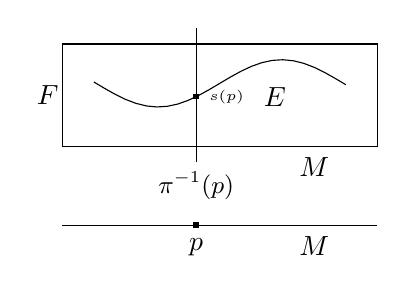
\begin{tikzpicture}[scale=1]
		\draw (-2,-0.3)--(2,-0.3)--(2,1)--(-2,1)--cycle;
		\node [label=left:$F$] (F) at (-1.8,0.35) {};
		\node [label=below:$M$] (M1) at (1.2,-0.2) {};
		\node [label=below:$M$] (M2) at (1.2,-1.2) {};
		\node [label=below:$E$] (E) at (0.7,0.7) {};
		\draw (-2,-1.3)--(2,-1.3);
		\node [fill=black, inner sep=1pt, label=below:$p$] (p) at (-0.3,-1.3) {};
		\draw [color=black, domain=-1.6:1.6] plot (\x,{0.3*sin(2*\x r)+0.5});
		%0.5-0.3*sin(0.6)=0.330607...
		\node [fill=black, inner sep=1pt, label=right:\tiny$s(p)$] (s) at (-0.3,0.3306) {};
		\draw (-0.3,-0.5)node[below]{\small$\pi^{-1}(p)$}--(-0.3,1.2);
	\end{tikzpicture}
	\caption{Trivial Bundle and its Section}
\end{figure}

一个纤维丛不一定有整体截面,但是一定有局部截面,因为纤维丛在局部都是平凡丛,而平反丛一定有截面,比如常值截面$s(x)=a\in F$。对于一个纤维丛,直观来看,就是在底流形$B$每一点$p$,都放一个$\pi^{-1}(p)\cong F$,而所谓的截面,就是在每一点$p$,都选定$\pi^{-1}(p)\cong F$中的一个元素,这其实也就是矢量场的基本想法。

反过来,如果给定了每一点的纤维,则我们有可能拼出一个纤维丛。切丛和余切丛正是如此定义的。

\para 流形$M$的切丛(tangent bundle) $TM$被在集合上被定义为
\[
	TM=\coprod_{x\in M}T_xM=\bigcup_{x\in M} \left\{x\right\}\times T_xM=\bigcup_{x\in M} \left\{(x, y)\vert\; y\in T_xM\right\}.
\]
余切丛(cotangent bundle)$T^*M$在集合上被被定义为
\[
	T^*M=\coprod_{x\in M}T^*_xM=\bigcup_{x\in M} \left\{x\right\}\times T^*_xM=\bigcup_{x\in M} \left\{(x, y)\vert\; y\in T_x^*M\right\}.
\]

\para 来看切丛,$M$显然是底流形,而$\pi$也可以显然地通过把$(p,v)\in TM$映射到$p\in M$来定义。剩下的,我们要赋予$TM$一个光滑流形结构,然后检验是否满足纤维丛的定义。

为此,对于$p\in M$,找一个坐标卡$(U,\varphi)$,在这张卡内,$T_qM$通过$\varphi_{*q}$同构于$\rr^n$,我们这样选取$\pi^{-1}(U)$上的微分结构,使得他通过$\id_U\times \varphi_*$光滑同胚于$U \times \rr^n$,这样$TM$就有了一个坐标卡$(\pi^{-1}(U),\varphi\times \varphi_*)$,于是他是一个光滑流形,也是一个以$M$为底,$\rr^n$为纤维的纤维丛。同样地,$T^*M$也是一个纤维丛。

\para 所以$U$上的光滑切矢量场就是$TM$的$U$上的一个光滑截面。

光滑切矢量场,局部依赖坐标$(U,\varphi)$,我们有$\varphi_*(X|_U)$在$\varphi(U)$上写作$Y^i \frac{\partial}{\partial x^i}$,那么通过逆映射$\varphi_*^{-1}$,我们就知道$X|_U$局部写作$X^i\partial_i$的形式。

现在我们自然提出反问题,设$v\in T_pM$是在$p$处的一个切矢量,我们是否可以(至少在局部)找到一个切矢量场$X$,使得$X_p=v$.

答案自然是有的,在局部,切矢量写作$X^i(p)(\partial_i)_p$,我们令$X^i$是常值的,则$x\mapsto X^i(x)(\partial_i)_x$就是一个我们所需的局部切矢量场。

\para 设$X$是一个$U$上的光滑矢量场,如果一条光滑曲线$\sigma:(-\epsilon,\epsilon)\to U$且$\sigma(0)=p$,满足$X(\sigma(t))=\dot{\sigma}(t)$,则称$\sigma$是$X$在$p$附近的一条积分曲线。

将矢量场局部写出来,$X(\sigma(t))=X^i(\sigma(t))\partial_t$,所以问题归结到了求解微分方程
\[
	\frac{\dd x^i\circ \sigma}{\dd t}(t)=X^i(\sigma(t)),
\]
他的初值为$\sigma(0)=p$。微分方程的(光滑)解在局部存在且唯一,所以我们得到了:

\para 在$p$附近,对$X$存在唯一的积分曲线$\sigma:(-\epsilon,\epsilon)\to U$.

\lem 设$X$是$U$上的光滑矢量场,如果$X_p\neq 0$,则存在一个$p$的邻域$V$,在$V$上存在一组坐标使得$X$可以写作$\partial_1$.

\proof
	完全是局部的结果,我们就在欧式空间里面证明,即找一组新的坐标来把$X=X^i\partial_i$变成$\partial'_1$. 此外,如果我们证明了可以写作$a \partial_1$,那么再令$x'$是$\partial x^1/\partial x'^1=a$的解(这个解积个分就出来了),那么自然就有$\partial'_1=a\partial_1$.

	不妨假设$X^1$在$p$的某个邻域不为零,现在我们来解常微分方程组
	\[
		\frac{\dd x^i}{\dd x^1}=\frac{X^n(x^1,\cdots,x^n)}{X^1(x^1,\cdots,x^n)},
	\]
	给定初值为$\{\varphi^i(0;v^2,\cdots,v^n)=v^i:2\leq i \leq n\}$,我们知道解$\{x^i=\varphi^i(x^1;v^2,\cdots,v^n)\}_{2\leq i \leq n}$局部存在且光滑依赖于初值$\{v^2,\cdots,v^n\}$以及$x^1$,所以我们选取新坐标$\{v^1,v^2,\cdots,v^n\}$使得
	\[
		\{x^1,x^2,\cdots,x^n\}=\{v^1,\varphi^2(v^1,\cdots,v^n),\cdots,\varphi^n(v^1,\cdots,v^n)\},
	\]
	容易计算他在$v^1=0$处的Jacobian行列式$\det(\partial x/\partial v)=1$,所以这是一个合理的坐标选取。

	最后,注意到$X^i=X^1 \dd x^i/\dd x^1=X^1 \dd x^i/\dd v^1$,所以
	\[
		X=X^i\partial_i=X^1 \frac{\dd x^i}{\dd v^1}\frac{\partial}{\partial x^i}=X^1\partial'_1.
	\]\qed

设$X$是$U$上的光滑矢量场,对$U$上的每一点$p$,都可以在$p$附近找到他的一条光滑积分曲线$\sigma_p$,上面的点$\sigma_p(t)$我们也记作$\sigma_t(p)$,这样我们就得到了一个新的一族映射$\{\sigma_t:U\to U\}$,当$t=0$的时候,$\sigma_0=\id$.这样的一族映射$\{\sigma_t\}$被称为矢量场$X$的\idx{流}。如果需要明确是那个矢量场的时候写作$\{\sigma^X_t\}$. 由微分方程解的唯一性可以发现$\sigma_t\circ \sigma_s=\sigma_{s+t}$.

对于一个矢量场,整体流的存在性是不能保证的,比如对$t=1$的时候,是否对每一个$p$变换$\sigma_1$都有意义?但是,至少在局部,我们可以保证在一定范围内的参数都是有意义的,对于局部的问题,这个存在性已经基本够使了。

\para 光滑流形$M$上的光滑矢量场$X$的支集被定义那些使$X$不为$0$的点集的闭包。如果$X$有紧支集,则$X$的流的参数可以全局定义到$\rr$上面去。特别地,如果流形是紧的,则对每一个光滑矢量场都成立。

设支集为$K$,找一个他的开覆盖,使得每一个开覆盖内$\sigma_t$都对某一个小区间$t\in (-\epsilon,\epsilon)$上有定义,由于紧,所以可以找到有限的子覆盖,所以在这些子覆盖里面,把最小的$\epsilon_{\text{min}}$挑出来,则在$K$上,对$t\in(-\epsilon_{\text{min}},\epsilon_{\text{min}})$,$\sigma_t$都有定义。现在对$p\notin K$定义$\sigma_t(p)=p$,容易检验$\epsilon_t$定义良好且还是光滑映射。最后,对$t>\epsilon_{\text{min}}$,我们可以从某个$t_0\in (-\epsilon_{\text{min}},\epsilon_{\text{min}})$反复复合$\sigma_{\epsilon_{\text{min}}/2}$,反之对$t<-\epsilon$亦然。

\para 现在我们将积分曲线的问题稍稍拓展一下,比如我们现在有两个矢量场$X$和$Y$,他们在每一点张成一个平面,类比于积分曲线,我们要问是否存在一个光滑曲面,使得这个曲面在每一点的切空间都是这俩矢量场张成的平面?

可以直接想象一下怎么处理这样的问题,直观来看,积分曲面可以由积分曲线拼成,即在$p$附近,$X$的一条一条积分曲线和$Y$的一条积分曲线编成一张网,这张网其实应该就在积分曲面上。因此积分曲面存在与否当且仅当这张网足够光滑,不能突然错开。此时的错开,就是说,从网格的一个端点处,沿着两条路径走到的终点处于积分曲面的两侧。

为简单见,我们看看这样一个曲边四边形。从$p$出发\footnote{这就意味着我们现在考虑的是局部问题,最后的解也应该被认为是局部的},沿着$X$的积分曲线走$s$,走到了$\sigma^X_s(p)$,再从这点出发,沿着$Y$的积分曲线走$t$,走到$\sigma^Y_t\circ\sigma^X_s(p)$.同样,从$p$出发,沿着$Y$的积分曲线走$t$,走到了$\sigma^Y_t(p)$,再从这点出发,沿着$X$的积分曲线走$s$,走到$\sigma^X_s\circ\sigma^Y_t(p)$。

这样我们就得到了弯曲的四边形,$p$是其中一个端点,但是一般来说,沿着两条路径并不会有相同的终点,即$p$的对角线方向的另一端点不存在,此时两条路径并不能闭合成一个弯曲的四边形。甚至,即使积分曲面存在,我们也不能得到一个闭合的四边形(网格),但是,如果沿着两条路径的终点是错开的,则积分曲面依然不存在。

实际上,因为$X$和$Y$的光滑,我们可以适当延长(或缩短)相比$s$和$t$小量的在一条路径上走的时间使得弯曲的四边形变成一个网格(此时局部积分曲面存在),或者,永远是错开的(此时局部积分曲面不存在)。

我们现在需要比较两条路径两个终点的差,在欧式空间里面,我们可以比较这两个点的距离。但是在流形上这样做是不方便的,我们可能连一个很直接的计算两个点距离的手段都没有。为了克服这个困难,我们可以采用“表示”的手段,取一个$U$上的光滑函数$f$,比较$f(\sigma^Y_t\circ\sigma^X_s(p))$和$f(\sigma^X_s\circ\sigma^Y_t(p))$。但光取一个$f$肯定是不够的,取而代之,我们可以取遍$U$上所有的光滑函数,如果我们关于所有的光滑函数都计算出了$f(\sigma^Y_t\circ\sigma^X_s(p))-f(\sigma^X_s\circ\sigma^Y_t(p))$(在$s$, $t$都很小时),那么就可以确认这两个坐标相差很小的程度。所以现在就是要计算在$s$, $t$都很小时的
\[
	g(s,t)=f(\sigma^Y_t\circ\sigma^X_s(p))-f(\sigma^X_s\circ\sigma^Y_t(p)).
\]

因为$g$是光滑函数,我们在$(0,0)$局部展开他,求导就可以得到系数。显然,他到二阶为止的导数都为$0$,并且$\partial_s^2g(0,0)=\partial_t^2g(0,0)=0$,所以他最低阶不为零的只可能是$\partial_s\partial_t g(0,0)$,这就是说,我们要求$\lim_{s,t\to 0}g(s,t)/st$.

\para 在$t$很小的时候,$f(\sigma_t^X p)=f(p)+tXf(p)+o(t^2)$.为了证明他,只要求$p$处的导数就行了,设$\sigma^X(t)$是$\sigma^X(0)=p$的$X$的积分曲线,则
\[
	\frac{\dd}{\dd t}\biggr|_{t=0}f(\sigma_t^X p)=\frac{\dd}{\dd t}\biggr|_{t=0}f\circ \sigma^X (t)=f_{* p}X=Xf(p).
\]

所以(暂时在记号上略去高阶项)
\[
	f(\sigma^Y_t\circ\sigma^X_s(p))=f(\sigma^X_s(p))+tYf(\sigma^X_s(p))=f(p)+sXf(p)+tY(\sigma^X_s\circ f(p)),
\]
以及
\[
	g(s,t)=sXf(p)+tY(\sigma^X_s\circ f(p))-tYf(p)-sX(\sigma^Y_t\circ f(p)),
\]
其中
\[
	Y(\sigma^X_s\circ f(p))-Yf(p)=sX(Y(f))(p),
\]
所以
\[
	g(s,t)=st\bigl(X(Y(f))(p)-Y(X(f))(p)\bigr),
\]
这就是说$\partial_s\partial_t g(0,0)=X(Y(f))(p)-Y(X(f))(p)$.

\para 定义两个矢量场$X$, $Y$的Lie括号为$[X,Y]$,他满足$[X,Y](f)=X(Y(f))-Y(X(f))$。

如果采用局部表示$X=X^i\partial_i$和$X=Y^i\partial_j$,则我们可以计算出
\begin{align*}
	[X,Y](f)&=X^i\partial_i(Y^j\partial_j f)-Y^i\partial_i(X^j\partial_j f)\\
	&=X^i\partial_iY^j\partial_j f-Y^i\partial_i X^j\partial_j f\\
	&=(X^i\partial_iY^j-Y^i\partial_i X^j)\partial_jf.
\end{align*}
因此,尽管形式上是二阶的,但$[X,Y]$还是一个切矢量场,局部写作$[X,Y]=(X^i\partial_iY^j-Y^i\partial_i X^j)\partial_j=(X(Y^j)-Y(X^j))\partial_j$.同时,我们可以将$[X,Y]_p$定义为$[X_p,Y_p]$,反过来,因为$X_p$和$Y_p$都可以扩张为局部的光滑切矢量场,所以对于任意的切矢量,我们都定义了一个双线性映射$[*,*]:T_pM\times T_pM\to T_pM$,他也被称为Lie括号。

\para 设$X_1$, $\cdots$, $X_k$是一族$U$上的切矢量场,记
	\[
		D=\bigl\{f_1X_1+\cdots+f_kX_k:\forall 1\leq i \leq k,\,\, f_i\in \calf(U)\bigr\},
	\]
	称他为$U$上的一个由$\{X_i\}$张成的分布。同样,我们也可以考虑一点处的分布,只要将上面的切矢量场改成切矢量,$\calf(U)$改成$\calf_p$即可。

\para 设点$p$附近有两个切矢量$X$和$Y$张成一个分布$D$,则局部积分曲面存在当且仅当$[X,Y]\in D$.

如果局部积分曲面存在,那么曲边四边形完全处于积分曲面上面,尽管沿着两条路径得到的终点可能不同,但是这两个点的连线(或者他的切矢量)应该在$s\to 0$, $t\to 0$的时候确定了一个切矢量(由于$X$和$Y$的光滑性,所以这个切矢量并不依赖于连线的选取),他处于积分曲面的切子空间(由$X_p$和$Y_p$张成)里面,且正比于$[X,Y]_p$,所以$[X,Y]_p=a(p)X_p+b(p)Y_p$.而$a$和$b$的光滑性是显然的。

如果不存在,就是说两个端点分处$X_p$和$Y_p$张成的切子空间两侧,所以两个点的连线确定的那个切矢量应该不在和$X_p$和$Y_p$张成的切子空间里,即$[X,Y]_p\neq aX_p+bY_p$.

\para 问题可以问得更广一点,设$X_1$, $\cdots$, $X_k$是一族切矢量场,他们是否(至少在局部)有积分“曲面”存在?回答是Frobenius定理:设$X_1$, $\cdots$, $X_k$在点$p$附近张成的分布为$D$,则局部存在积分“曲面”当且仅当对任意的$i$和$j$成立$[X_i,X_j]\in D$。

当然,这个结论可以更加形式地证明他,如果不信任上面的直观想法,则可以参看任何一本微分流形的教材,我这里就略去了。

\para 令$\varphi$是流形$M$上的光滑可逆变换,设矢量场$X$的流为$\sigma_t$,则$\varphi_*X$的流为$\varphi\circ \sigma_t\circ\varphi$.

设在$p$处的切矢量为$X_p$,经过$p$的$X$的积分曲线为$\sigma(t)$,使用变换$\varphi$,变成了$q=\varphi(p)$,$q$处的切矢量$\varphi_{*p}X_p=(\varphi_*X)_q$以及积分曲线$\varphi(\sigma(t))=\varphi(\sigma_t q)=\varphi\circ\sigma_t\circ \varphi^{-1}(p)$.此即结论。

所以,$\varphi_*X=X$当且仅当$\varphi\circ \sigma^X_t=\sigma^X_t\circ \varphi$成立。

\para 直接的计算,我们有:
	\[
		[X,Y]=\lim_{t\to 0}\frac{1}{t}\bigl(Y-(\sigma_t^X)_*Y\bigr).
	\]

所以,如果$\sigma_t^X$和$\sigma_s^Y$可交换,即$\sigma_t^X\circ \sigma_s^Y=\sigma_s^Y\circ \sigma_t^X$,则$(\sigma_t^X)_*Y=Y$以及$[X,Y]=0$.

\para 设$\varphi:M\to N$是一个光滑映射,$X$和$Y$分布是$M$和$N$上的光滑函数,称他们是$\varphi$相关的,如果$\varphi_*X(f)=Y(f)\circ \varphi$对任意光滑函数$f$成立。局部来看,$X_p(f\circ \varphi)=Y_{\varphi(p)}(f)$.

若$X_1$与$Y_1$是$\varphi$相关的,$X_2$与$Y_2$是$\varphi$相关的,则$[X_1,X_2]$和$[Y_1,Y_2]$是$\varphi$相关的,因为
\begin{align*}
	\varphi_*[X_1,X_2](f)&=X_1(X_2(f\circ \varphi))-[1\leftrightarrow 2]\\
	&=X_1(Y_2(f)\circ\varphi)-[1\leftrightarrow 2]\\
	&=Y_1(Y_2(f))\circ \varphi-[1\leftrightarrow 2]\\
	&=[Y_1,Y_2](f)\circ \varphi.
\end{align*}
因为对于一个同胚而言,$\varphi_*(X)$被定义为$p\mapsto \varphi_{*\varphi^{-1}(p)}X_{\varphi^{-1}(p)}$,或者$\varphi(p)\mapsto \varphi_{*p}X_p$,这就是说
\[
	X_p(f)=\varphi_*(X)_{\varphi(p)}(f),
\]
因此$X$与$\varphi_*X$是$\varphi$相关的。


\para 令$\varphi$是$U$上的光滑同胚$\varphi:U\to \varphi(U)$,$X$和$Y$是$U$上的矢量场,则在$U$上$\varphi_{*}[X,Y]=[\varphi_{*}X,\varphi_{*}Y]$.

因此,作为局部的同胚,$\sigma_s^X$可以适用
\[
	(\sigma_s^X)_*[X,Y]=[X,(\sigma_s^X)_*Y]=\lim_{t\to 0}\frac{1}{t}\bigl((\sigma_s^X)_*Y-(\sigma_{s+t}^X)_*Y\bigr)=\frac{\dd}{\dd t}\biggr|_{t=s}(\sigma_t^X)_*Y.
\]

如果$[X,Y]=0$,则$(\sigma_t^X)_*Y$是一个常矢量(局部来看,系数为常数),因此$Y$在$(\sigma_t^X)_*$作用下不变,这就是说$Y=(\sigma_t^X)_*Y$,于是$\sigma_t^X$和$\sigma_s^Y$可交换.

\para 综上,$[X,Y]=0$当且仅当$\sigma_t^X$和$\sigma_s^Y$可交换。

既然流是可交换的,那么以前我们谈的那个曲边四边形总是可以闭合的,所以这种情况下积分流形局部肯定存在,因为在局部我们可以一块一块曲边四边形拼起来。由于显然的$[\partial_i,\partial_j]=0$,如果我们能够选取局部坐标使得一族矢量场$\{X_i:1\leq i \leq k\}$变成$\{\partial_i:1\leq i \leq k\}$,则积分曲面存在。那么什么时候$\{X_i\}$是可以变成$\{\partial_i\}$呢?答案前面已经有了,$[X_i,X_j]\in D$,分布$D$由$\{X_i\}$生成。当然,这可以直接证明,所以这也是证明积分曲面存在性的一种思路。

最后给个例子,$n$维欧式空间,$\{\partial_i:1\leq i \leq k\}$的可能的积分曲面$\{x_i=c_i:k+1\leq i \leq n\}$,其中$c_i$是常数。如果这个积分曲面还是连通的,设$\pi$是往最后$n-k$个坐标的投影,则$\pi_*\partial_i=0$,其中$1\leq i \leq k$,因此$(\pi\circ i)_*=0$,其中$i$是积分流形往欧式空间的嵌入,此时由积分流形的连通性,$\pi\circ i$是常值映射。此时的积分流形就是上面的$\{x_i=c_i:k+1\leq i \leq n\}$.

\section{Cotangent Vector Field}

\para 设$U\osub M$,$U$上的光滑余切矢量场(或者叫做一个1-形式)是余切丛在$U$上的一个光滑截面。余切矢量场$\omega$都可以写作$\omega=a_i\dd x^i$,其中$a_i$是$V$上的实值函数,而$\dd x^i$在不同的点分属不同的余切空间。因为是光滑余切矢量场,所以$\{a_i\}$在点$p$是光滑函数。

一个余切矢量场和一个切矢量场之间存在作用$\omega(X)=X(\omega)$可以得到一个光滑函数,具体来说就是在每一点$p$,$\omega_p(X_p)\in \rr$.

% \para 正如切矢量场,对余切矢量场$\omega$,光滑性也有如下判据:$\omega$是光滑的,当且仅当$\omega(X)$是光滑的对$U$上的任意光滑切矢量场$X$成立。

\para 设$f$是$U$上的光滑函数,显然$\dd f$是一个$U$上的光滑余切矢量场。记$U$上的光滑函数的集合为$\Omega^0(U)$,记$U$上的光滑余切矢量场的集合为$\Omega^1(U)$,则$\dd: \Omega^0(U)\to \Omega^1(U)$.

下面我们要把Frobenius定理改写成余切矢量场的形式,这就变成了经典的Pfaff方程,正是当年关于Pfaff方程的研究,Cartran第一次提出了(高阶)外微分和微分形式的概念(我们现在只谈了一阶的情况),在他那里,1-形式之间的乘法被定义成反对称的。从前一节谈论Frobenius定理来看,Pfaff方程是一个关于积分曲面的问题,所以从这个角度来看,反对称的来由归根结底是为了积分。

\para 称一个1-形式$\omega$是完全可积的,如果存在两个光滑函数$f$和$g$使得$\omega=f\dd g$,此时$f$被称为$\omega$的积分因子。

1-形式的完全可积性联系着所谓的首次积分问题。设$f$是一个光滑函数且$\dd_p f$处处不为零,则$f(p)=a$(如果解存在)决定了$M$中的一个正则子流形$N_a$(有时候叫做一个曲面)。再设$X$是$M$内的光滑矢量场,则$\dd f(X)=0$恒成立当且仅当处处成立$X_p\in T_pN_{f(p)}$。

实际上,任取一点$p\in M$,只要检验$X_p(f)=0$即可,选一条$N_{f(p)}$上的一条光滑曲线$c$,使得$c(0)=p$且$c'(0)=X_p\in T_pN_{f(p)}$,由于$f(c(t))=f(p)$恒成立,对其在$t=0$处求导就得到了$\dd_pf(X_p)=X_p(f)=0$.反过来,如果在一点处$X_p\notin T_pN_{f(p)}$,则$X_p(f)\neq 0$。

固定$f$,将所有$\dd f(X)=0$的$X$拿出来,他组成一个$n-1$维的分布,$\{N_a\}$就是这个分布的一族积分流形,因为$X$在每一点都完全位于经过那一点的某个$N_a$的切空间内。我们称$N_a=\{p\in M:f(p)=a\}$是Paffa方程$\dd f=0$的解。从上面来看,一个Paffa方程要有解,那么解应该是一个积分曲面才是,即,Paffa方程$\omega=0$的解是使得$\omega(X)=0$的所有的$X$的积分曲面。

现在假设一个1-形式$\omega$是完全可积的,即他可以写作$\omega=f\dd g$,那么Paffa方程$\omega=0$等价于$\dd g=0$,这就确定了一个积分曲面。

\para 设$\omega$是一个1-形式,记分布$\ker \omega$是由满足$\omega(X)=0$的所有$X$张成的一个分布。记$\ker(\omega_1,\cdots,\omega_r)=\cap_{i=1}^r\ker \omega_i$.

% 则这个$\omega$完全可积当且仅当$\ker \omega$存在积分曲面。

\para 在局部,对任意一个分布$L$,存在一族余切矢量场$\{\omega_i:1\leq i \leq r\}$使得$L=\ker(\omega_1,\cdots,\omega_r)$.

实际上,一个分布在局部,和他在流形一点处(一个矢量空间内)是很相似的。设$L$是一个分布,由$r$个光滑的切矢量场$\{X_i:1\leq i \leq r\}$张成,则在局部,我们可以找到$n-r$个光滑矢量场$\{X_i:r+1\leq i \leq n\}$,使得$\{X_i:1\leq i \leq n\}$处处线线性无关。依然在局部,我们可以找到与其对偶\footnote{即满足$\omega_i(X_j)=\delta_{ij}$.}的1-形式$\{\omega_i:1\leq i \leq n\}$,那么那些使得$\omega(X)$对$X\in L$成立的1-形式局部由$\{\omega_i:r+1\leq i \leq n\}$张成。因此,局部上,一个分布$L$可以写作$L=\ker(\omega_{r+1},\cdots,\omega_n)$,等价地,可以写作一个Paffa方程组$\{\omega_i=0:r+1\leq i \leq n\}$.

因为局部存在积分曲面的充要条件是任取$X$, $Y\in D$满足$[X,Y]\in D$,所以如果$L=\ker(\omega_{r+1},$ $\cdots$, $\omega_n)$存在积分曲面,应该有$\omega_i([X,Y])=0$。

\para 设$\omega=f\dd g$,其中$f$和$g$是光滑函数,则对一般的光滑矢量场$X$, $Y$成立。
\begin{equation}
\begin{split}
	\omega([X,Y])=f\dd g([X,Y])&=f [X,Y](g)\\
	&=fX(Y(g))-fY(X(g))\\
	&=X(fY(g))-X(f)Y(g)-Y(fX(g))+Y(f)X(g)\\
	&=X(\omega(Y))-Y(\omega(X))-\bigl(X(f)Y(g)-Y(f)X(g)\bigr).
\end{split}
\end{equation}

对于$X(f)Y(g)-Y(f)X(g)$,我们可以将其改写为$\dd f(X)\dd g(Y)-\dd g(X)\dd f(Y)$,因为这是关于$X$和$Y$的双线性函数,我们可以引入一个张量$\dd f\otimes \dd g$使得$\dd f\otimes \dd g(X,Y)=\dd f(X)\dd g(Y)$,则
\[
	\dd f(X)\dd g(Y)-\dd f(Y)\dd g(X)=\dd f\otimes \dd g(X,Y)-\dd g\otimes \dd f(X,Y)=(\dd f\otimes \dd g-\dd g\otimes \dd f)(X,Y).
\]
记$\dd f\wedge \dd g=\dd f\otimes \dd g-\dd g\otimes \dd f$,其中的$\wedge$被称为\idx{楔积},记$D(f\dd g)=\dd f\wedge \dd g$,则式(\theequation)变成了
\[
	D(f\dd g)(X,Y)=X(\omega(Y))-Y(\omega(X))-\omega([X,Y]).
\]
从式子右端来看,$\dd f\wedge \dd g(X,Y)$并不依赖于$\omega$的具体形式$\omega=f\dd g$。实际上,任意一个1-形式$\omega$可以写作$\omega=\sum_i f_i\dd g_i$,所以对于一般的情况,式(\theequation)应该写作
\[
	\sum_iD(f_i\dd g_i)(X,Y)=X(\omega(Y))-Y(\omega(X))-\omega([X,Y]).
\]
如果我们把$D$看做线性算子,则对于任意一个1-形式,我们都定义了一个线性算子,满足
\begin{equation}
	D(\omega)(X,Y)=X(\omega(Y))-Y(\omega(X))-\omega([X,Y]).
	\label{eq:1.3}
\end{equation}

\para 当然,我们也可以反过来通过式\eqref{eq:1.3}来定义$D(\omega)$,顺序在这里不是紧要的。紧要的是,$D(\omega)$决定了$\ker \omega$是否容许一个积分曲面。这是因为,如果$X$, $Y\in \ker \omega$,则式\eqref{eq:1.3}变成了
\[
	D(\omega)(X,Y)=-\omega([X,Y]),
\]
所以$D(\omega)(X,Y)=0$当且仅当$[X,Y]\in \ker \omega$.

这正是Cartan当年提出微分形式时候的处境,那时候,他从Frobenius和Darboux那里知道了,不同的Pfaff形式的等价条件就联系在一个bilinear covariant上面,而这个bilinear covariant就是我们这里的$D(\omega)$.

从这个角度来看,正因为有Frobenius定理,或者更本质一点,我们需要把积分曲线拼成积分曲面,我们需要考察两个矢量场$X$和$Y$的Lie括号$[X,Y]$,而这个Lie括号的反对称性来自于我们比较两条路径。现在,这种反对称性反应在了1-形式之间的楔积,使得他构成了一个(吃掉两个矢量场的)反对称函数。所以,从Cartan这里,反对称性的来源应该是为了处理积分曲面的存在性,而由$[X,Y]$自然诱导出来的。

\para 外代数的复习在附录,对于矢量空间$V$的$k$-次外代数记做$\Omega^k(V)$。在流形上的一点$p$处,记$\Omega_p^k=\Omega^k(T_pM)$,则$\Omega_p^1=T_p^*M$.类似切丛和余切丛,我们可以使用$\Omega_p^k$拼出一个$k$-形式丛$\Omega^k$。

\para 在$U$上的一个光滑$k$-形式被定义为$\Omega^k$在$U$上的一个光滑截面。所有$U$上的光滑$k$-形式的集合记做$\Gamma(\Omega^k,U)$.显然,$U$上的光滑函数可以看成一个光滑$0$-形式,一个光滑余切矢量场是一个光滑1-形式。如果$\omega$是一个光滑$1$-形式,则$D(\omega)$是一个光滑$2$-形式。下面我们所称的形式都是光滑的,我们将省略光滑二字。

\para 设分布$L$由$\{X_i:1\leq i \leq r\}$张成,且$L=\ker(\omega_{r+1},\cdots,\omega_n)$,如果$D(\omega)(X_i,X_j)=0$成立,则$D(\omega)$可以写作\[
	D(\omega)=\sum_{i=r+1}^n \psi_i\wedge \omega_i,
\]
其中$\psi_i$是一次微分式.

实际上,局部地$\{\omega_i:1\leq i\leq n\}$构成一组基,则
\[
	\dd \omega = \sum_{i=r+1}^n \psi_i\wedge w_i +\sum_{i,j=1}^r a_{ij}\omega_i\wedge \omega_j,
\]
其中$\psi_i$是一次微分式,而$a_{ij}$是光滑函数,且关于指标是反对称的。因为$\omega_i(X_j)=\delta_{ij}$,所以
\[
	0=\dd \omega(X_i,X_j)=\sum_{p,q=1}^r a_{pq}\omega_p\wedge \omega_q(X_i,X_j)=\sum_{p,q=1}^r a_{pq}(\delta_{ip}\delta_{jq}-\delta_{jp}\delta_{iq})=2a_{ij}.
\]

\para 设分布$L$由$\{X_i:1\leq i \leq r\}$张成,且$L=\ker(\omega_{r+1},\cdots,\omega_n)$,则$L$存在积分曲面当且仅当,
\[
	D(\omega_i)=\sum_{j=r+1}^n \psi_{ij}\wedge \omega_i
\]
对每一个$i$都成立。

\para 特别地,设分布$L=\ker(\omega)$,则局部积分曲面存在的充分必要条件是$D(\omega)=\psi\wedge \omega$,再或者$D(\omega)\wedge \omega=0$.则也就是$\omega$完全可积的充分必要条件。

\para \label{dd=0}可以计算得到$D(\dd f)=0$。实际上,从\eqref{eq:1.3}
\[
	D(\dd f)(X,Y)=X(Y(f))-Y(X(f))-[X,Y](f)=[X,Y](f)-[X,Y](f)=0,
\]
对任意的矢量场$X$, $Y$都成立。

\section{Exterior Derivative}

函数$f$的支集$\supp(f)$被定义为$\{x\in M:f(x)\neq 0\}$的闭包。下面关于单位分解的引理的证明看附录,这里仅摘录定义和引理:

\textbf{\eqref{POUdef}} 单位分解:设$\{U_\alpha\}_{\alpha\in I}$是$M$的一个开覆盖,如果存在可数个光滑函数$g_i\in \calf(M)$满足:

\no{1} 对于任意的$x\in M$和$i\in I$,都有$0\leq g_i(x)\leq 1$.

\no{2} 对每个$g_i$,都存在一个${\alpha_i}$使得$\supp(g_i)\subset U_{\alpha_i}$.

\no{3} 集族$\{\supp(g_i)\}$局部有限,即任取$p\in M$,存在$p$的邻域$U$使得$U$只和集族$\{\supp(g_i)\}$中的有限个集合相交非空。

\no{4} 因为上一个性质,所以在一点累加$g_i$时,只有有限项非零。我们最后的要求就是$\sum_i g_i=1$.

则称$\{g_i\}$是从属于开覆盖$\{U_\alpha\}_{\alpha\in I}$的一个单位分解。

\textbf{\lemref{POU}} 流形$M$上的每一个开覆盖都存在从属于他的单位分解。

\para \label{unit} 设$V\subset U$,且$\bar{V}\subset U$,则$M-\bar{V}$和$U$构成$M$的一个开覆盖,我们可以找到$h$, $g\in \calf(M)$使得$h+g=1$处处成立,且$h|_{M-U}=0$以及$g|_{\bar{V}}=0$,因此$h|_{\bar{V}}=1$.

\para 在很久很久以前,对$U$上的一个光滑函数$f$,我们定义了外微分$\dd$,使得$\dd f$是一个1-形式,而在上一节,我们对$U$上的一个1-形式$\omega$,定义了$D$使得$D(\omega)$是一个2-形式。更一般地,我们希望可以定义如下一个算符
\[
	\dd_k:\Gamma(\Omega^k,U)\to \Gamma(\Omega^{k+1},U),
\]
使得$\dd_0=\dd$,$\dd_1=D$。我们将$\{\dd_k\}$统称为外微分算符,统一记做$\dd$,他完成了一个$k$-形式到一个$(k+1)$-形式的转变。

所以,我们对于线性算符$\dd$,需要满足如下性质,

\no{1} 对于光滑函数$f$,$\dd f$就是我们前面定义的微分。

\no{2} 任取光滑函数$f$,$\dd^2 f=\dd (\dd f)=0$,这来自于\eqref{dd=0},也是暗示$\dd$作用在1-形式上应该和$D$差不多。

\no{3} 作为微分算符的Leibniz法则:设$\omega$是$k$-形式,则
\[
	\dd(\omega\wedge \eta)=\dd \omega \wedge \eta +(-1)^k \omega\wedge \dd\eta,
\]
其中$(-1)^k$的出现来自楔积的交换。这个Leibniz法则我们已经在计算$D(f\dd g)$和$\dd(fg)$的时候遇到过了。

\para \label{localform}先假设$\dd$在$U$上是存在的。若$\omega$是$V\osub U$上的$k$-形式,设$W$是$U$的一个开子集且$V$真包含$\overline{W}$.那么正如\eqref{unit}说的,可以找一个单位分解$h$,使得$h|_{\overline{W}}=1$以及$h|_{U-W}=0$,利用他就可以定义一个$U$上的光滑$k$-形式$h\omega$(他在$V$外为零,在$W$内等同于$\omega|_W$)。

\para \label{regular}设$U$是流形$M$上的开集且$V\osub U$,则存在$V$的一个开覆盖$\{W_\alpha\}_{\alpha\in I}$使得对每个$\alpha$成立$\overline{W_\alpha}\subset V$.

实际上这就是分离公理之一,正则性的直接推论。流形$M$是局部紧的Hausdorff空间,所以他是正则的。而对于正则空间内的每一个点$p$,已知邻域$V$,我们可以找到一个邻域$W_p\subset V$使得$\overline{W_p}\subset V$.然后遍历$p$,就找到了开覆盖$\{W_p\}_{p\in V}$.

\para \label{localpro}设$V\osub U$,如果$\omega|_V=0$,则$(\dd \omega)|_V=0$,即$\dd$是一个局部算符。

利用\eqref{regular}找一个$V$的开覆盖,我们只要证明对开覆盖中的一个开集$W$,$(\dd \omega)|_{W}=0$即可。同\eqref{localform}利用单位分解找一个光滑函数$h$,则$h\omega$在$U$上恒为零,所以
\[
	0=\dd (h\omega)=\dd h \wedge \omega +h\dd \omega
\]
限制在$W$上,$h|_{W}=1$且$(\dd h)|_{W}=0$(利用$\dd h$是一个微分这一个事实),所以$(\dd \omega)|_{W}=0$.

\pro \label{localdef}利用\eqref{localpro},设$V\osub U$,如果$U$上存在外微分形式$\dd$,则他诱导出了$V$上的一个外微分形式$\dd_V$。并且,再设$W\osub W$,则$\dd$在$W$上诱导的$\dd_W$和$\dd_V$在$W$诱导的$\dd_{VW}$是相同的。此外$(\dd_V \omega)|_W=\dd_W (\omega|_W)$对任意的$V$上的$k$-形式$\omega$成立。

\proof 和上面的想法差不多,利用\eqref{regular},我们可以找一个开覆盖。然后在每个开覆盖中的开集$W$上,同\eqref{localform}利用单位分解找一个光滑函数$h_W$,使得$h_W\omega$成为$U$上的光滑$k$-形式,定义$(\dd_V \omega)|_{W}=\dd (h_W\omega)|_{W}$.

设$W'$是开覆盖中的另外的开集,且$W\cap W'\neq \varnothing$。由于$(h_W\omega)|_{W\cap W'}=(h_{W'}\omega)|_{W\cap W'}$,因为\eqref{localpro},则
\[
	\dd (h_W\omega)|_{W\cap W'}=\dd (h_{W'}\omega)|_{W\cap W'},
\]
所以
\[
	((\dd_V \omega)|_{W})|_{W\cap W'}=((\dd_V \omega)|_{W'})|_{W\cap W'}
\]
保证了$(\dd_V \omega)|_W$在相交的开集上是相同的,这就使得我们可以黏结他们定义出一个$V$上的$(k+1)$-形式$\dd_V \omega$. 容易检验$\dd_V$满足所有外微分的性质。至于$\dd_W=\dd_{VW}$,从构造来看,这是显然的。

最后我们来检验等式$(\dd_V \omega)|_W=\dd_W (\omega|_W)$,对$W$利用\eqref{regular}找个开覆盖,在每一个开集$X$上,把上式左边限制到$X$上即$((\dd_V \omega)|_W)|_X=(\dd_V \omega)|_X=\dd(h_X\omega)$,同样,右边限制到$X$上即$(\dd_W (\omega|_W))|_X=\dd(h_X\omega|_W)=\dd(h_X\omega)$,所以等式成立。\qed

\para 设$W\subset V$是$U$中的开集,以及$\rho^k_{VW}$和$\rho^{k+1}_{VW}$分别是$k$-形式和$(k+1)$-形式的限制映射。设$\omega$是$V$上的任意$k$-形式,由于$\rho^{k+1}_{VW}\circ \dd_V (\omega)=(\dd_V \omega)|_W=\dd_W (\omega|_W)=\dd_W \circ \rho^k_{VW}(\omega)$,所以我们有
\[
\dd_W\circ \rho^k_{VW}=\rho^{k+1}_{VW}\circ \dd_V.
\]
换句话说,$\dd$诱导了预层$U\mapsto \Gamma(\Omega^k,U)$和预层$U\mapsto \Gamma(\Omega^{k+1},U)$间的自然变换(或者叫做函子间的态射)。

\para 容易证明,以$p$的邻域$W$赋予包含而成的归纳系,
\[
	\Omega_p^k=\varinjlim_{W\ni p}\Gamma(\Omega^k,W),\quad \Omega_p^{k+1}=\varinjlim_{W\ni p}\Gamma(\Omega^{k+1},W),
\]
以及有到点上的限制映射$\rho^k_{Wp}$和$\rho^{k+1}_{Wp}$。则colimt的泛性质,如下交换图告诉我们$\dd_p:\Omega_p^k\to \Omega_p^{k+1}$存在。
\[
	\xymatrix{
	&&\ar[dl]^{\rho^k_{Vp}}\Gamma(\Omega^k,V)\ar[dd]^{\rho^k_{VW}}\ar@/_/[lld]_{\rho^{k+1}_{Vp}\circ \dd_V} \\
	\Omega_p^{k+1}&\ar@{-->}[l]_(0.3){\dd_p}\Omega_p^{k}&\\
	&&\ar[ul]_{\rho^k_{Wp}}\Gamma(\Omega^k,W)\ar@/^/[llu]^{\rho^{k+1}_{Wp}\circ \dd_W}
	}
\]
以后,方便起见,即使$\omega$只是$U$的开集$V$上的$k$-形式的时候,我们依旧用$\dd \omega$来标记$\dd_V \omega$.这当然也就意味着,在记号上,$\dd(\omega|_W)=(\dd\omega)|_W$.

\pro 在流形$M$上,外微分算子$\dd$存在且唯一。

\proof 有了上面这些铺垫,我们只要在局部证明其唯一存在即可,然后把他拼起来,就像Proposition \eqref{localdef}做的那样。首先证明局部唯一性,为此当然假设$\dd$是存在的。在局部,我们找一族坐标,对于$k$-形式,他写作
\[
	\omega=\sum_{i_1,\cdots ,i_k} a_{i_1\cdots i_k}\dd x^{i_{1}}\wedge\cdots\wedge x^{i_{k}},
\]
由于$\dd$是线性算子,我们可以只考虑
\[
	\omega=a\dd x^{1}\wedge\cdots\wedge \dd x^{k}.
\]

由于Leibniz法则,
\[
	\dd \omega=\dd a \wedge \dd x^{1}\wedge\cdots\wedge \dd x^{k}+a\dd(\dd x^{1}\wedge\cdots\wedge \dd x^{k}),
\]
对于第二项,使用Leibniz法则,以及$x^1$是光滑函数,所以有的$\dd^2 x^1=0$,于是
\[
	\dd(\dd x^{1}\wedge\cdots\wedge \dd x^{k})=-\dd x^{1}\wedge\dd(\dd x^{2}\wedge\cdots\wedge \dd x^{k}),
\]
这样进行下去就知道他是零。于是
\[
	\dd \omega=\dd a \wedge \dd x^{1}\wedge\cdots\wedge \dd x^{k},
\]
这样$\dd$在局部的表现完全由他那些性质唯一决定,唯一性得证。

剩下的存在性,我们就把上面的过程反过来,在局部的$k$-形式写作
\[
	\omega|_U=\sum_{i_1,\cdots ,i_k} a_{i_1\cdots i_k}\dd x^{i_{1}}\wedge\cdots\wedge x^{i_{k}},
\]
则定义其外微分为
\[
	\dd(\omega|_U)=\sum_{i_1,\cdots ,i_k} \dd a_{i_1\cdots i_k}\wedge\dd x^{i_{1}}\wedge\cdots\wedge x^{i_{k}},
\]
不难检验外微分的性质都可以得到满足。这样我们就在局部证明了外微分的存在性。

最后,由于$(\dd(\omega|_U))|_{U\cap V}=\dd(\omega|_U|_{U\cap V})=\dd(\omega|_V|_{U\cap V})=(\dd(\omega|_V))|_{U\cap V}$,所以我们可以将局部定义的外微分算子粘起来得到流形$M$上的一个外微分算子。由于外微分算子的局部唯一性,所以也就得到了他的整体唯一性。\qed

\pro 虽然是一个很简单的命题,但是很重要:$\dd^2=0$.

\proof 局部对单项式证明即可,设$\omega=a\dd x^{1}\wedge\cdots\wedge \dd x^{k}$,则
\[
	\dd \omega=\dd a\wedge \dd x^{1}\wedge\cdots\wedge \dd x^{k}
\]
以及
\[
	\dd^2 \omega=\dd^2 a\wedge \dd x^{1}\wedge\cdots\wedge \dd x^{k}-\dd a\wedge \dd^2 x^{1}\wedge\cdots\wedge \dd x^{k}+\cdots=0.
\]
\qed

\para 我们将$\dd \omega=0$的形式$\omega$称为闭形式,将$\omega=\dd \eta$的形式$\omega$称为恰当形式,则这一命题告诉我们,恰当形式一定是闭形式,反之不一定。我们定义$H^k(M)=\ker(d_k)/\im(d_{k-1})$为流形$M$的第$k$个上同调群,其中模的运算是看做加法群的商群运算,这个$H^k(M)$即表征了闭的$k$-形式在除去一个恰当形式后的等价类。此外约定当$k<0$的时候,$H^k(U)=0$.

当$k=0$的时候,$H^0(U)$就是$\mathrm{ker}\left(\dd:\calf(U)\to\Omega^1(U)\right)$.如果$U$是连通的,$\dd f=0$就昭示着$f$在恒为常数,$H^0(U)$就是这些函数构成的矢量空间。那么如果有着不同的连通分支,那么$H^0(U)$就是在在各个连通分支上为常数(整体不一定是一样的)的那些函数构成的矢量空间。而他的维度就是连通分支的个数。

下一节将会提到一点,上同调群是流形拓扑的表征,他是一个拓扑范畴到交换群范畴的反变函子,对于同伦等价的拓扑空间,有着同构的上同调群。所以这是一个拓扑不变量,如果我们可以把两个拓扑空间的上同调群计算出来得到他们不同构,则这两个拓扑空间必然不同伦。流形的上同调群也被称为de Rham上同调,他是上同调群的一个典型,这里$\dd$是自然的边缘算子的对偶,而楔积是自然的cup product(比起同调,上同调里的cup product是比“对偶”部分多出来的东西)。

\para 正如\eqref{eq:1.3}我们看到的,对$1$-形式$\omega$,我们有
\[
	\dd(\omega)(X,Y)=X(\omega(Y))-Y(\omega(X))-\omega([X,Y]),
\]
类似地,对$k$-形式$\omega$,经过一些不算复杂的计算,我们可以证明
\[
\begin{split}
	\dd(\omega)(X_1,\cdots,X_{k+1})=&\sum_{i=1}^{k+1}(-1)^{i+1}X_i\bigl(\omega(X_1,\cdots,\hat{X_i},\cdots,X_{k+1})\bigr)\\
	&+\sum_{1\leq i<j\leq k+1}(-1)^{i+j}\omega\bigl([X_i,X_j],X_1,\cdots,\hat{X_i},\cdots,\hat{X_j},\cdots,X_{k+1}\bigr),
\end{split}
\]
其中
\[
	\omega\bigl(X_1,\cdots,\hat{X_i},\cdots,X_{k+1}\bigr)=\omega\bigl(X_1,\cdots,X_{i-1},X_{i+1},\cdots,X_{k+1}\bigr),
\]
以及
\[
\begin{split}
	\omega\bigl([X_i,X_j],X_1,\cdots,\hat{X_i},\cdots,&\hat{X_j},\cdots,X_{k+1}\bigr)=\\
	&\omega\bigl([X_i,X_j],X_1,\cdots,X_{i-1},X_{i+1},\cdots,X_{j-1},X_{j+1},\cdots,X_{k+1}\bigr),
\end{split}
\]
就是说,头上带帽等于把他去掉。这个式子可以反过来拿来定义$\dd$,而且确实是一个坐标无关的定义。我们并没有那么做,因为就实际计算而言,更多时候我们并不会把形式作用在所有的光滑切矢量场上。

\para 设$f:M\to N$,我们前面已经谈到了,这个$f$在0-形式,即光滑函数之间诱导了一个$f^*$(被称为一个拉回),即$f^*g=g\circ f$. 对于$1$-形式,由\eqref{f*d=df*},我们知道了$f^*\dd g=\dd (f^* g)$,对比矢量场之间$f_*$的定义还需要$f$是单射,这里1-形式之间的$f^*$则没有这个限制。

\para 通过$(f^*\omega)_p=\omega_{f(p)}\bigl(f_{*p}(X_1)_p,\cdots,f_{*p}(X_k)_p\bigr)$,我们可以定义出$k$-形式之间的$f^*$.

\para 所以,很容易检验,$f^*(\omega\wedge \eta)=(f^*\omega)\wedge (f^*\eta)$.

实际上,这个式子也可以反过来定义$k$-形式之间的$f^*$.可是这样定义可能会遇到一些技术性问题,比如一个$k$-形式大范围来说是否一定能写成一些比较低阶的形式楔积并线性组合而成?如果不,怎么通过上式定义?这个问题的回答是,类似\eqref{localpro},拉回是一个局部算符,即如果$\omega$在局部为零,则$f^*\omega$也在局部为零,所以我们可以不从大范围考虑这个问题。

\para 按照上面这种定义方式,假设$f^*$存在,则$f^*$是一个局部算符。

首先注意到$f^*(h\omega)=(f^*h)(f^*\omega)$。设$\omega$在$U$上为零,利用\eqref{regular},我们可以找一个$U$开覆盖。然后在每个开覆盖中的开集$W$上,同\eqref{localform}利用单位分解找一个光滑函数$h_W$,则按照上式$f^*(h_W\omega)$只可能在$\overline{W}$内不为零,因此,如果$\omega$在$U$上为零,则$h_W\omega$就恒为零,所以$(f^*h_W)(f^*\omega)=f^*(h_W\omega)=0$. 由于$f^*h_W=h_W\circ f$在$f^{-1}(W)$内等于$1$,所以$(f^*\omega)|_{f^{-1}(W)}=0$,遍历开覆盖,我们就得到了$(f^*\omega)|_{f^{-1}(U)}=0$.

特别地,如果$\omega_1$和$\omega_2$在$U$上相同,则$0=(f^*(\omega_1-\omega_2))|_{f^{-1}(U)}=(f^*\omega_1)|_{f^{-1}(U)}-(f^*\omega_2)|_{f^{-1}(U)}$,这就意味着$f^*\omega_1$和$f^*\omega_2$在局部相同,此即黏合条件。

我们这里不再重复类似$\dd_U$诱导出$\dd_V$的过程,以及这些$f^*_U$什么的和限制映射之间的关系,统统直接记做$f^*$,则$f^*(\omega_{U})=(f^* \omega)_{f^{-1}(U)}$。因为局部来说$k$-形式确实可以写成一些比较低阶的形式楔积并线性组合而成,以及我们已经对$0$-形式和$1$-形式定义了拉回,则局部的$k$-形式的拉回可以使用我们的定义递归地定义出来,那么剩下的只要拼起来就好,而这正需要黏合条件。

最后,这样定义的$f^*$在一点诱导出的$f^*_p$(类似$\dd$到$\dd_p$)可以验证和$1$-形式间已经存在的$f^*_p$用张量积诱导出来的映射是相同的。

\para 设$f:M\to N$,则$f^*(\dd \omega)=\dd (f^*\omega)$.实际上,我们只要局部对单项式证明即可,设$\omega=a\dd x^{1}\wedge\cdots\wedge \dd x^{k}$,则$\dd \omega=\dd a\wedge \dd x^{1}\wedge\cdots\wedge \dd x^{k}$,以及
\[
	f^*(\dd \omega)=(f^*\dd a)\wedge f^*(\dd x^{1}\wedge\cdots\wedge \dd x^{k})=\dd (f^*a)\wedge \dd f^*(x^{1})\wedge\cdots\wedge \dd f^*(x^{k})=\dd (f^*\omega).
\]

因为$f^*$将恰当形式映射成恰当形式,即$f^*(\im \dd_N)\subset \im \dd_M$,所以他诱导了两个流形上同调群之间的同态$f^*:H^k(N)\to H^k(M)$.

\section{Introduction to de Rham Cohomology}

我们这节将目标放在$\rr^n$中的de Rham上同调。

\para 一系列矢量空间和上面的线性映射$A\xrightarrow{f}B\xrightarrow{g}C$称为正和列,就是说$\ker g=\mathrm{Im} f$.而$0\to A\xrightarrow{f}B$
就是说$f$是单射,而$B\xrightarrow{g}C\to 0$就是说$g$是满射。而正和列
\[
0\to A\xrightarrow{f}B\xrightarrow{g}C\to 0
\]
称为短正合列。

\para 一个矢量空间和线性映射链$A^*=\{A_i,\dd_i\}$
\[
	\cdots\to A^{i-1}\xrightarrow{\dd^{i-1}}A^i\xrightarrow{\dd^i}A^{i+1}\to \cdots
\]
称为链复形,如果对于任意的$i$都有$\dd^i \circ \dd^{i+1}=0$.当对任意的$i$都有$\ker \dd^i=\mathrm{Im}\, \dd^{i-1}$,则这个链复形称为正和的。

\para 很容易看到,$\Omega^*(M)$和外微分算子$\dd$构成一个链复形。那么同样,对于任意的链复形都可以定义上同调群$H^p(A^*)=\ker (\dd^p)/\mathrm{Im} (\dd^{p-1})$,其中的元素同样用等价类符号$[a]$记。

\para 如果在两条链的每一个对应链的对象之间,譬如说$A_i$和$B_i$之间,存在线性映射$f^i$,那么自然就在两条链之间引入了一个映射$f:A^*\to B^*$,需要交换图如下:
	\[
	\xymatrix{
		\cdots\ar[r]&A^{p-1}\ar[r]^{\dd_A^{p-1}}\ar[d]^{f^{p-1}}&A^p\ar[r]^{\dd_A^p}\ar[d]^{f^{p}}&A^{p+1}\ar[r]\ar[d]^{f^{p+1}}&\cdots\\
		\cdots\ar[r]&B^{p-1}\ar[r]^{\dd_B^{p-1}}&B^p\ar[r]^{\dd_B^p}&B^{p+1}\ar[r]&\cdots
	}
	\]
从交换图可以看到,应该满足$\dd^{p}_B\circ f^p=f^{p+1}\circ \dd^{p}_A$.既然在链复形之间引入了映射,则他诱导了上同调群之间的映射。通过$f^*([a])=[f^p(a)]$,我们诱导了$f^*=H^p(f):H^p(A^*)\to H^p(B^*)$.

\para 链复形也可以构成一个链,尤其重要的是短正合列$0\to A^*\xrightarrow{f}B^*\xrightarrow{g}C^*\to 0$.链的短正和列就是当对任意的$p$都有短正合列$0\to A^p\xrightarrow{f^p}B^p\xrightarrow{g^p}C^p\to 0$.

\pro 链复形的短正合列$0\to A^*\xrightarrow{f}B^*\xrightarrow{g}C^*\to 0$引入了上同调群的正合列$H^p(A^*)\xrightarrow{f^*}H^p(B^*)\xrightarrow{g^*}H^p(C^*)$.

\proof 其实就是证明$\ker g^*=\mathrm{Im}\, f^*$.首先证明$\mathrm{Im}\, f^* \subset \ker g^*$,任取$[a]\in H^p(A^*)$,我们有
\[
g^*\circ f^*([a])=[g^p\circ f^p(a)]=[0]=0.
\]
这是从正合列$A^p\xrightarrow{f^p}B^p\xrightarrow{g^p}C^p$中得知的。

然后证明$\ker g^*\subset \mathrm{Im}\, f^*$.这就是说,任意的$g^*[b]=0$的$[b]$都可以找到$[a]$使得$f^*[a]=[b]$.

因为对任意的$p$有$0=g^*[b]=[g^p(b)]$,因此存在一个$c$使得$g^p(b)=\dd^{p-1}_C(c)$,而$g^{p-1}$又是满射,所以可以找到$b'$使得$g^{p-1}(b')=c$,因此用交换图变换
\[
g^p(\dd^{p-1}_B(b'))=d^{p-1}_C(g^{p-1}(b'))=g^p(b).
\]

所以$g^p(b-\dd^{p-1}_B(b'))=0$,所以存在$a$使得$f^p(a)=b-\dd^{p-1}_B(b')$。现在只要证明这个$a$确实在$\ker \dd^p_A$里面就可以了。为此只要证明$\dd^p_A a=0$就可以,但是因为$f^{p+1}$是单射,所以也等价于证明$f^{p+1}\circ \dd^p_A (a)=0$.用交换图变换
\[
f^{p+1}\circ \dd^p_A (a)=\dd^p_B\circ f^p (a)=\dd^p_B(b-\dd^{p-1}_B(b'))=\dd^p_B(b)=0.
\]
因为$a$确实在$\ker \dd^p_A$里面,所以他在$H^p(A^*)$里面对应了一个等价类$[a]$,成立$f^*[a]=[b]$.\qed

\para 链复形的短正和列还引入了其他两个正合列。对于链复形的短正合列$
0\to A^*\xrightarrow{f}B^*\xrightarrow{g}C^*\to 0$,定义$\partial^*:H^p(C^*)\to H^{p+1}(A^*)$为线性映射
\[
	\partial^*([c])=\left[(f^{p+1})^{-1}\left(\dd^p_B\left((g^p)^{-1}(c)\right)\right)\right].
\]

$\partial^p$即交换图
	\[
		\xymatrix{
			&0\ar[d]&0\ar[d]&0\ar[d]&\\
			\cdots\ar[r]&A^{p-1}\ar[r]^{\dd_A^{p-1}}\ar[d]^{f^{p-1}}&A^p\ar[r]^{\dd_A^p}\ar[d]^{f^{p}}&A^{p+1}\ar[r]\ar[d]^{f^{p+1}}&\cdots\\
			\cdots\ar[r]&B^{p-1}\ar[r]^{\dd_B^{p-1}}\ar[d]^{g^{p-1}}&B^p\ar[r]^{\dd_B^p}\ar[d]^{g^{p}}&B^{p+1}\ar[r]\ar[d]^{g^{p+1}}&\cdots\\
			\cdots\ar[r]&C^{p-1}\ar[r]^{\dd_B^{p-1}}\ar[d]&C^p\ar[r]^{\dd_B^p}\ar[d]\ar[ruu]&C^{p+1}\ar[r]\ar[d]&\cdots\\
			&0&0&0&
		}
	\]
中的斜线。这里就不证明这是良定义的了。因此,链复形的短正合列$0\to A^*\xrightarrow{f}B^*\xrightarrow{g}C^*\to 0$诱导了上同调群的正合列
\[
\begin{split}
&H^p(B^*)\xrightarrow{g^*}H^p(C^*)\xrightarrow{\partial^*}H^{p+1}(A^*),\\
&H^p(C^*)\xrightarrow{\partial^*}H^{p+1}(A^*)\xrightarrow{f^*}H^{p+1}(B^*).
\end{split}
\]

\theo \label{longexact}
链复形的短正合列$0\to A^*\xrightarrow{f}B^*\xrightarrow{g}C^*\to 0$引入了上同调群的正合列
\[
\cdots\to H^p(A^*)\xrightarrow{f^*}H^p(B^*)\xrightarrow{g^*}H^p(C^*)\xrightarrow{\partial^*}H^{p+1}(A^*)\xrightarrow{f^*}H^{p+1}(B^*)\to\cdots.
\]

\pro \label{directsum} 链复形可以谈论直和,即是对链中每一个矢量空间进行直和。那么从$\ker$和$\mathrm{Im}$对于直和的显然性质,我们有$H^p(A^*\oplus B^*)=H^p(A^*)\oplus H^p(B^*)$.

$\Omega^*(U)$和外微分算子$\dd$构成一个链复形,下面的定理给出了有关于欧氏空间两个开集和他们的并与交的短正合列。

\theo 设$U_1$和$U_2$是$\rr^n$中的开集,记$i_\nu:U_\nu \to U_1 \cup U_2$和$j_\nu:U_1\cap U_2 \to U_\nu$是嵌入,则有如下的短正合列:
\[
0\to \Omega^p(U_1\cup U_2)\xrightarrow{I^p}\Omega^p(U_1)\oplus\Omega^p(U_2)\xrightarrow{J^p}\Omega^p(U_1\cap U_2)\to 0.
\]
其中$I^p(\omega)=(i_1^*(\omega),i_2^*(\omega))$, $J^p(\omega_1,\omega_2)=j_1^*(\omega_1)-j_2^*(\omega_2)$.

\proof 先证明$I^*$是单射,这就是说除了$I^*(\omega)=0$只有解$\omega=0$.

设$\varphi$是$\rr^n$中的开集的嵌入,则对于任意的$p$-形式$\dd x_I=\dd x_{i_1}\wedge\dots\wedge\dd x_{i_p}$都有$\varphi^* \dd x_I =\dd x_I$,因此
\[
\varphi^*\omega=\varphi^*\sum_If_I\dd x_I=\sum_If_I\circ\varphi \dd x_I.
\]

现在证明$J^*$是一个满射。将单位分解应用到$U_1$和$U_2$上面取,存在$p_\nu$为定义在$U_1\cup U_2$上的光滑函数,而他的非零点集包含于$U_\nu$,且$p_1(x)+p_2(x)=1$.

设$f$定义在$U_1\cap U_2$上。定义$U_1$上的光滑函数$f_1$,他在$U_1\cap U_2$上的限制为$f(x)p_2(x)$和$U_2$上的光滑函数$f_2(x)$,他在$U_1\cap U_2$上的限制为$-f(x)p_1(x)$.那么在$U_1\cap U_2$上$f_1(x)-f_2(x)=f(x)$.

所以任选一个$U_1\cap U_2$上的$p$-形式$\omega$,系数$f_I$都可以定义出$f_{1,I}$和$f_{2,I}$,并且在$U_1\cap U_2$上满足$f_{1,I}-f_{2,I}=f$,因此也定义了两个$\omega_1$和$\omega_2$得到$J^p(\omega_1,\omega_2)=\omega$.

那么$I^*(\omega)=0$就是说$i_1^*(\omega)=i_2^*(\omega)=0$,这就是说$f_I\circ i_1=f_I\circ i_2=0$,但是由于$U_1$和$U_2$是$U_1\cup U_2$的一个开覆盖,所以这就等价于$f_I=0$,所以$\omega=0$.

然后证明$\ker J^p=\mathrm{Im}\, I^p$.分两个包含。

\no{1} $\mathrm{Im}\, I^p\subset \ker J^p$
\[
J^p\circ I^p(\omega)=j_2^*\circ i_2^*(\omega)-j_1^*\circ i_1^*(\omega)
\]
但其实$i_2\circ j_2=i_1\circ j_1$,所以$J^p\circ I^p(\omega)=0$.

\no{2} $\ker J^p\subset \mathrm{Im}\, I^p$

设$\omega_1=\sum_I f_I \dd x_I\in \Omega^p(U_1)$和$\omega_2=\sum_I g_I \dd x_I\in \Omega^p(U_2)$,从$J^p(\omega_1,\omega_2)=0$我们有$j_1^*(\omega_1)=j_2^*(\omega_2)$,这就是说$f\circ j_1=g\circ j_2$,或者说$f$和$g$在$U_1\cap U_2$恒等。我们可以构成一个光滑函数$h_I$,他在$U_1$上的限制恒等于$f_I$,而$U_2$上恒等于$g_I$.那么
\[
I^p\left(\sum_Ih_I\dd x_I\right)=(\omega_1,\omega_2).
\]\qed

将Theorem \eqref{longexact} 和 Proposition \eqref{directsum} 应用到上面这个定理。就得到下面这个定理。

\theo Mayer-Vietoris列:
设$U_1$和$U_2$是$\rr^n$中的开集,则有如下的正合列:
\[
\cdots\to H^p(U_1\cup U_2)\xrightarrow{I^*}H^p(U_1)\oplus H^p(U_2)\xrightarrow{J^*}H^p(U_1\cap U_2)\xrightarrow{\partial^*}H^{p+1}(U_1\cup U_2)
\to \cdots
\]
其中$I^*([\omega])=(i_1^*([\omega]),i_2^*([\omega]))$,$J^*([\omega_1],[\omega_2])=j_1^*([\omega_1])-j_2^*([\omega_2])$.

如果$U_1\cap U_2=\varnothing$,那么$H^p(U_1\cap U_2)=0$.所以
\[
0\xrightarrow{\partial^*} H^p(U_1\cup U_2)\xrightarrow{I^*}H^p(U_1)\oplus H^p(U_2)\xrightarrow{J^*}0,
\]
那么$I^*$既单又满,故而是个同构。

如果我们已知$U_1$和$U_2$的上同调群,那么通过Mayer-Vietoris列我们就有可能计算他们的并或者交的上同调群。

\para \label{homotopy}两个连续函数$f$, $g:X\to Y$被称为\idx{同伦}的,就是说存在一个连续函数$H:X\times [0,1]\to Y$使得$H(0,x)=f(x)$以及$H(1,x)=g(x)$.同伦是等价关系,就是说,如果还有$h$和$f$同伦,则$g$和$h$也同伦。一个空间$X$是可缩的,如果$\id_X$同伦于映到自身的常值映射。比如$\rr^n$或者与他同胚的开实心球$D^n$都是可缩的。

两个集合$X$和$Y$称为同伦等价的,如果存在$f:X\to Y$和$g:Y\to X$满足$f\circ g$和$\id_Y$同伦以及$g\circ f$和$\id_X$同伦。下面我们尝试说明,上同调群是同伦不变量。即在同伦意义下,上同调群是同构的。

\lem 光滑函数的同伦的一个技术性引理(见单位分解的附录):在欧氏空间背景下,任何一个连续映射都同伦于一个光滑映射。如果两个光滑函数$f_1$, $f_2:U\to V$是同伦的,则存在光滑函数$F:U\times \rr\to V$满足$F(x,0)=f_1(x)$和$F(x,1)=f_2(x)$.

\pro 两条链复形和两个映射$f$, $g:A^*\to B^*$如果对每一个$p$都存在线性映射$s^p:A^p \to B^{p-1}$满足
\[
\dd_B^{p-1}s^p+s^{p+1}\dd_A^p=f^p-g^p:A^p\to B^p.
\]
则$f^*=g^*$.这样的两个映射被称为链同伦的。

\proof 对任意的$[a]\in H^p(A^*)$,我们有$\dd_A^p(a)=0$,所以
\[
(f^*-g^*)[a]=[(f^p-g^p)a]=[\dd^{p-1}_Bs^p(a)+s^{p+1}\dd_A^p(a)]=[\dd^{p-1}_Bs^p(a)],
\]
而$\dd^{p-1}_Bs(a)$显然被等价为0,所以$f^*=g^*$.\qed

\pro 如果两个光滑函数$f$, $g:U\to V$是同伦的,则$
f^*$, $g^*:\Omega^*(V)\to \Omega^*(U)$是链同伦的,即$f^*=g^*$。

\proof 利用我们的技术性引理,由于$f$, $g:U\to V$是同伦的,所以存在光滑函数$F:U\times \rr \to V$使得$F(x,0)=f(x)$和$F(x,1)=g(x)$.

注意到任意的$U\times \rr$上的$p$-形式可以写作
\[
\omega=\sum_If_I(x,t)\dd x_I+\sum_J g_J(x,t)\dd t\wedge \dd x_J.
\]
让$\varphi_0:x\mapsto (x,0)$和$\varphi_1:x\mapsto (x,1)$,则$F\circ \varphi_0=f$和$F\circ \varphi_1=g$,且将上面的形式分别拉回到
\[
\varphi_0^*\omega=\sum_I f_I(x,0)\dd x_I,\quad
\varphi_1^*\omega=\sum_I f_I(x,1)\dd x_I.
\]

现在我们需要构造一个$S^p:\Omega^p(U\times \rr)\to \Omega^{p-1}(U)$使得
\[
(\dd \circ S^p+S^{p+1}\circ \dd)(\omega)=(\varphi_1^*-\varphi_0^*)(\omega),
\]
如果这样,对于任意$U$中的形式我们有
\[
(\dd \circ S^p+S^{p+1}\circ \dd)(F^*\omega)=(\varphi_1^*-\varphi_0^*)(F^*\omega)=((F\circ \varphi_1)^*-(F\circ \varphi_0)^*)(\omega)=(g^*-f^*)(\omega),
\]
而最左边又有
\[
(\dd \circ S^p\circ F^*+S^{p+1}\circ F^* \circ \dd)(\omega)
\]
所以只要定义$s^p=S^p\circ F^*$,这就是链同伦。

为此定义
\[
S^p(\omega)=\sum_J\left(\int_0^1g_J(x,t)\dd t\right)\dd x_J.
\]\qed

利用这个命题,我们可以知道,同伦等价对应到上同调群就有了上同调群的同构,因此上同调群只依赖于同伦型。

\para 由于对于可缩开子集$0^*=\id^*$,所以如果$U\subset \rr^n$可缩,那么$U$上的闭形式是恰当形式。这被称为Poincar\'{e}引理,通过他,我们知道可缩开集$U$的上同调群如下,$H^0(U)=\rr$,而对于$p>0$,则为$H^p(U)=0$.

\para 用Mayer-Vietoris列计算$H^{p}(\rr^2-\{0\})$.

设$U_1$为去掉正实轴(包括原点)的平面,$U_2$为去掉负实轴(包括原点)的平面,因此$U_1\cup U_2=\rr^2-\{0\}$.两者都是可缩的,所以由Poincaré引理可以知道,$H^0(U_1)=H^0(U_2)=\rr$以及如果$p>0$有$H^p(U_1)=H^p(U_2)=0$.

注意到$U_1\cap U_2$为去掉实轴的平面$I_1\cup I_2$,两个部分无交且各自可缩,所以
\[
H^p(U_1\cap U_2)=H^p(I_1\cup I_2) \cong H^p(I_1)\oplus H^p(I_2) =\begin{cases}
\rr\oplus\rr&,p=0;\\
0&,p>0.
\end{cases}
\]
而$\rr^2-\{0\}$是连通的,所以$H^0(\rr^2-\{0\})=\rr$.

当$p>0$的时候,代入Mayer-Vietoris列
\[
H^p(U_1\cap U_2)\xrightarrow{\partial^*}H^{p+1}(U_1\cup U_2)\xrightarrow{I^*}H^{p+1}(U_1)\oplus H^{p+1}(U_2)\xrightarrow{J^*}H^{p+1}(U_1\cap U_2),
\]
头尾通过计算都为$0$,所以
\[
H^{p+1}(\rr^2-\{0\})=H^{p+1}(U_1\cup U_2)\cong H^{p+1}(U_1)\oplus H^{p+1}(U_2)=0.
\]
这就是说,平面挖一个洞的$2$阶以上的上同调群为$0$.

现在考察一阶$\rr^2-\{0\}$的上同调群,由于负阶都为$0$,所以
 \[
0\to H^0(U_1\cup U_2)\xrightarrow{I^*}H^0(U_1)\oplus H^0(U_2)\xrightarrow{J^*}H^0(U_1\cap U_2)\xrightarrow{\partial^*}H^{1}(U_1\cup U_2)\to 0
\]
或者
 \[
0\to \rr\xrightarrow{f}\rr\oplus\rr\xrightarrow{g}\rr\oplus\rr\xrightarrow{h}H^{1}(\rr^2-\{0\})\to 0.
\]
由于$f$是单射而且正和性给出$\ker g = \mathrm{Im}\,f$,所以$\ker g =\rr$,而由线性代数基本定理,有$\mathrm{Im}\,g \cong \rr$,因此正合列给出$\ker h \cong \rr$,而因为$h$是满射,所以根据同构基本定理$H^{1}(\rr^2-\{0\})\cong(\rr\oplus\rr)/\ker h \cong \rr$.

综上,\[H^{p}(\rr^2-\{0\})\cong
\begin{cases}
\rr&,p=0,1;\\
0&,p>1.
\end{cases}\]

\para  同样是Mayer-Vietoris列的算例。将$\rr^n$看做$\rr^{n+1}$的子空间,设$A$是$\rr^n$中的闭子集,则
\[
\begin{cases}
H^{p+1}(\rr^{n+1}-A)\cong H^p(\rr^n-A),&\text{when}\,p>1,\\
H^{1}(\rr^{n+1}-A)\cong H^0(\rr^n-A)/\rr,&\\
H^{0}(\rr^{n+1}-A)\cong \rr.&
\end{cases}
\]

通过归纳法可以得到
\[H^{p}(\rr^n-\{0\})\cong
\begin{cases}
\rr&,p=0,n-1;\\
0&,\text{otherwise}.
\end{cases}\]
这个结论可以用来证明$\rr^m$和$\rr^n$之间不存在同胚,如果存在,将同胚调整为$0$映射到$0$,而由于同胚将产生上同调群间的同构,所以$H^{p}(\rr^n-{0})$与$H^{p}(\rr^m-{0})$对于任意$p$都是同构的,但这不可能。

由于当$n>0$的时候,$S^{n-1}$和$\rr^n-\{0\}$同胚(当然也自然同伦等价),所以我们也计算出了球面的上同调群为
\[H^{p}(S^{n})\cong
\begin{cases}
\rr&,p=0,n;\\
0&,\text{otherwise}.
\end{cases}\]

上面一些计算出的上同调群可以产生许多有名经典的拓扑结论,比如Jordan-Brouwer分割定理,Brouwer不动点定理等。最简单的,比如$S^n$和$S^m$在$n\neq m$时候不同胚。

\section{Integration}

\para 对于$p\geq 0$,以及$\rr^{p+1}$中的$p+1$个矢量$\{v_i:0\leq i\leq p\}$满足$\{v_i-v_0:1\leq i\leq p\}$是一个线性无关组,我们定义$p$-单形为
\[
	[v_0,\cdots,v_p]=\left\{\sum_{i=0}^p a_iv_i\in \rr^{p+1}:\sum_{i=1}^p a_i=1,\text{and each } a_i\leq 0\right\}.
\]
一个标准$p$-单形为$[e_0,\cdots,e_p]$,其中$\{e_i\}_{0\leq i \leq p}$是$\rr^{p+1}$的标准基,可以看到,每一个$p$单形都和标准$p$-单形同胚。但是,流形$M$上的一个(光滑)$p$-单形是指一个(光滑)映射$\sigma:[v_0,\cdots,v_p]\to M$,这是光滑曲线的自然推广,因为流形上的光滑曲线就是一个1-单形。我们常说沿着某条曲线积分,这里我们就将推广到沿着某个单形积分。

一个0-单形是一个点$1$,一个1-单形$[v_0,v_1]$是一个线段,端点为$v_0$和$v_1$,一个2-单形是一个三角形,他的三个顶点位于$v_0$, $v_1$和$v_2$,一个3-单形位于四维空间,不太好想,但是从上面的类比,他应该是一个四面体,顶点位于$v_0$, $v_1$, $v_2$和$v_3$.记$M$上全部$p$-单形生成的自由Abel群(或者称$\zz$-模)为$C_p(M)$,当然,这里两个单形之间的加法的定义意义似乎还不太明朗。我们将$C_p(M)$中的元素称为$p$-链,显然,一个$p$-单形就是一个$p$-链。

\para 一个$p$-单形内的每一个点都可以写作$\sum_{i=0}^p a_iv_i$的形式,我们称某个$(p-1)$-边界是指某个$a_i=0$的情况,一个$(p-1)$边界是自然的$(p-1)$-单形,记做$[v_0,\cdots,\hat{v}_i,\cdots,v_p]$。显然,一个$p$-单形有$p+1$个边界,比如一个三角形,是一个2-单形,有三条边。

对于流形$M$上的一个$p$-单形$\sigma:[v_0,\cdots,v_p]\to M$,定义他的第$(i+1)$个边缘为一个$(p-1)$-链$\sigma|_{[v_0,\cdots,\hat{v}_i,\cdots,v_p]}$。

\para 在流形$M$上,定义边缘算子$\partial:C_p(M)\to C_{p+1}(M)$:对单项式,
\[
	\partial \sigma=\sum_{i=0}^p (-1)^i\sigma|_{[v_0,\cdots,\hat{v}_i,\cdots,v_p]}.
\]
对一般的$\sigma=\sum_i n_i \sigma_i$,定义$\partial \sigma =\sum_i n_i \partial \sigma_i$.

\para 我们有$\partial^2=0$.

\proof 直接对单项式计算
\[
\begin{split}
	\partial^2 \sigma&=\sum_{i=0}^p (-1)^i\partial\sigma|_{[v_0,\cdots,\hat{v}_i,\cdots,v_p]}\\
	&=\sum_{0\leq i<j\leq n}^p (-1)^{i+j-1}\bigl(\sigma|_{[v_0,\cdots,\hat{v}_i,\cdots,\hat{v}_j,\cdots,v_p]}-\sigma|_{[v_0,\cdots,\hat{v}_i,\cdots,\hat{v}_j,\cdots,v_p]}\bigr)=0.
\end{split}
\]\qed

$\partial^2=0$和$\dd^2=0$是如此的相似!实际上,我们可以定义$H_k(M)=\ker\partial/\im\partial$,这就是流形$M$的第$k$个奇异同调群。这里不展开,我们暂时的目标还是积分。

\para 由于每一个$[v_0,\cdots,v_p]$都同胚与标准$p$-单形,所以,在同胚意义下,以标准$p$-单形为定义域的流形上的$p$-单形与定义域为花式的$[v_0,\cdots,v_p]$的流形上的$p$-单形应该是一样多的。所以我们可以限定,流形上的$p$-单形的定义域为标准$p$-单形。

\para 由于$[v_0,\cdots,v_p]$里面的点写作$\sum_i a_i v_i$,注意到$\sum_i a_i=1$,我们可以将其改写为
\[
	\sum_{i=0}^pa_iv_i=\left(1-\sum_{i=1}^pa_i\right)v_0+\sum_{i=1}^pa_iv_i=v_0+\sum_{i=1}^pa_i(v_i-v_0),
\]
所以,除去一个平移$v_0$,我们完全可以由$\sum_{i=1}^pa_i(v_i-v_0)$确定一个$p$-单形。显然,他们是光滑同胚的。所以对于$M$上的$p$-单形,我们在光滑同胚意义下,还可以假设定义域为
\[
	\Delta^p=\left\{(a_1,\cdots,a_p):a_i\geq 0\text{ and }\sum_i a_i\leq 1\right\},
\]
这时候,$\sigma:\Delta^p\to M$常常会写作$\sigma(a_1,\cdots,a_p)$.

此时,对于边缘算子,这种约定下,符号要变得复杂一些,记
\[
	k^p_0(a_1,\cdots,a_{p})=\left(1-\sum_{i=1}^{p-1}a_i,\cdots,a_{p}\right),
\]
当$i>0$时,
\[
	k^p_i(a_1,\cdots,a_{p})=(a_1,\cdots,a_{i-1},0,a_{i+1},\cdots,a_{p}),
\]
以及$\sigma^i=\sigma\circ k^p_i$,则
\[
	\partial\sigma=\sum_{i=0}^p(-1)^i \sigma^i,
\]
不难检验,$\partial^2=0$还是成立的,以后我们就采用这种符号约定。

\para 设$\omega$是$\rr^n$中的$n$-形式,写作$f\dd x^1\wedge\cdots\wedge \dd x^n$,则我们定义他在区域$A$上的积分算符为线性函数
\[
	\int_A \omega=\int_A f \dd x^1\cdots\dd x^n,
\]
有时候为了省空间,我们以$\Int_A$来记$\int_A$. 并且,反过来,我们也将欧式空间里的$n$-重积分写作对微分形式积分的样子
\[
	\int_A f \dd x^1\cdots\dd x^n=\int_A f\dd x^1\wedge\cdots\wedge \dd x^n.
\]

有了这个定义,我们可以重写积分变量替换公式为
\[
	\int_{\varphi(A)}\omega=\pm\int_A \varphi^*\omega,
\]
其中当$\det(\varphi_*)>0$的时候取正,反之取负。

\para 设$\sigma$是一个$M$上的0-单形,即一个点$\sigma(0)\in M$,定义在$\sigma$上的积分为$\Int_\sigma \omega=\omega(\sigma(0))$.

\para 对于$p\leq 1$的情况,设$\sigma:\Delta^p\to M$是一个$M$上的一个$p$-单形,这里$p>0$,那么$\sigma$诱导了一个拉回映射$\sigma^*$,我们定义一个$p$-形式$\omega$在$\sigma$上的积分如下:
\[
	\int_\sigma \omega=\int_{\Delta^p} \sigma^*\omega,
\]
注意到等式右边就是一个$\rr^{p}$内对$p$-形式的积分,这个积分上面我们已经定义了。

当我们在一条链上积分的时候,比如$c=\sum_{i} n_i \sigma_i$,我们定义
\[
	\int_c \omega=\sum_i n_i \int_{\sigma_i} \omega.
\]
此时,单形之间加起来成链在积分的意义下清楚了不少。

\para 设$f:M\to N$是一个光滑映射,设$\sigma$是$M$上的一个单形,则$f\circ \sigma$是$N$上的一条单形,那么对$N$上的$p$-形式
\[
	\int_{f\circ\sigma} \omega = \int_{\Delta^p}(f\circ \sigma)^*\omega= \int_{\Delta^p}\sigma^*\circ f^*(\omega)=\int_{\sigma}f^*\omega.
\]
这推广了重积分变量替换公式。

\theo 微积分基本定理:设$c$是$M$上的一个1-链,而$f$是$M$上的一个光滑函数,则
\[
	\int_{\partial c} f=\int_c \dd f.
\]
对于$c$是一个1-单形的时候,这个定理翻译成我们熟知的语言即$\int_a^b \dd f=f(b)-f(a)$,而两边对于$c$都是线性的,所以上述定理对链依然成立。

\theo 著名的Stocks定理(还能叫微积分基本定理):设$c$是$M$上的一个$p$-链,而$\omega$是$M$上的一个$(p-1)$-单形,则
\[
	\int_c \dd \omega=\int_{\partial c} \omega.
\]

这是两个(一个)极伟大的定理,尽管证明他并不是特别困难。他的重要性无需强调,每一个做过定积分(包括曲面积分等)计算的人都知道他多么有用。

\proof 对于$p=1$的情况,这就是微积分基本定理,所以我们下面假设$p\leq 2$.由于积分对链是线性的,所以我们只要对一个单形去证明就可以了,即
\[
	\int_{\sigma} \dd \omega=\int_{\partial \sigma} \omega,
\]
利用积分的定义,我们把单形拉回到欧式空间里面,证明几乎就可以在欧式空间里面进行,即
\[
	\int_{\Delta^p} \sigma^*(\dd \omega)=\sum_{i=0}^p(-1)^i\int_{\Delta^{p-1}} (\sigma^i)^*\omega=\sum_{i=0}^p(-1)^i\int_{\Delta^{p-1}} (k^p_i)^*\circ \sigma^*(\omega).
\]

我们假设
\[
	\sigma^*\omega=\sum_{i=1}^pa_i\dd x^1\wedge\cdots\wedge\widehat{\dd x^i}\wedge\cdots \dd x^p,
\]
所以等式左边写作
\[
\begin{split}
	\int_{\Delta^p} \sigma^*(\dd \omega)=\int_{\Delta^p} \dd(\sigma^* \omega)&=\sum_{i=1}^p\int_{\Delta^{p}} \dd a_i\wedge \dd x^1\wedge\cdots\wedge\widehat{\dd x^i}\wedge\cdots\wedge\dd x^p\\
	&=\sum_{i=1}^p\int_{\Delta^{p}} (-1)^{i-1}\partial_i a_i\dd x^1\wedge\cdots \wedge\dd x^p.
\end{split}
\]

现在来看右边,由于
\[(k^p_0)^*(x^j)=
\begin{cases}
	1-\sum_{i=1}^{p-1}x^i,& j =1;\\
	x^{j-1},& j>1,
\end{cases}\quad
(k^p_i)^*(x^j)=
\begin{cases}
	x^j,& 1\leq j \leq i-1;\\
	0,& j=i;\\
	x^{j-1},& i+1\leq j \leq p.
\end{cases}
\]
所以
\[
\begin{split}
	\sum_{i=0}^p(-1)^i\int_{\Delta^{p-1}}& (k^p_i)^*(a_j\dd x^1\wedge\cdots\wedge\widehat{\dd x^j}\wedge\cdots \dd x^p)\\
	&=(-1)^{j-1}\int_{\Delta^{p-1}} (a_j\circ k^p_0)\dd x^1\wedge\cdots \wedge\dd x^{p-1}+(-1)^j\int_{\Delta^{p-1}} (a_j\circ k_j^p)\dd x^1\wedge\cdots \wedge\dd x^{p-1},
\end{split}
\]
对右侧第一项做一个适当的变量替换$\varphi^i$如下
\[
	\varphi^i(x)=\begin{cases}
		x,& i=1;\\
		\bigl(1-\sum_{i=1}^{p-1}x^i,x^2,\cdots,x^{p-1}\bigr),& i=2;\\
		\bigl(x^2,\cdots,x^{i-1},1-\sum_{i=1}^{p-1}x^i,x^{i+1},\cdots,x^{p-1}\bigr),& 2<i\leq p.
	\end{cases}
\]
容易证明$\varphi^i(\Delta^{p-1})=\Delta^{p-1}$以及$\det ((\varphi^i)_*)=1$,所以,由重积分变量替换公式,我们得到
\[
\begin{split}
	\sum_{i=0}^p&(-1)^i\int_{\Delta^{p-1}} (k^p_i)^*(a_j\dd x^1\wedge\cdots\wedge\widehat{\dd x^j}\wedge\cdots \dd x^p)\\
	=&(-1)^{j-1}\int_{\Delta^{p-1}} a_j\left(x^1,\cdots,x^{j-1},1-\sum_{i=1}^{p-1}x^i,x^{j},\cdots,x^p\right)\dd x^1\wedge\cdots \wedge\dd x^{p-1}+\\
	&(-1)^{j}\int_{\Delta^{p-1}}a_j(x^1,\cdots,x^{j-1},0,x^{j},\cdots,x^p)\dd x^1\wedge\cdots \wedge\dd x^{p-1},
\end{split}
\]
所以最后我们只需要证明
\[
\begin{split}
	\int_{\Delta^{p}}\partial_i a_i\dd x^1\wedge\cdots \wedge\dd x^p=
	&\int_{\Delta^{p-1}} a_j\left(x^1,\cdots,x^{j-1},1-\sum_{i=1}^{p-1}x^i,x^{j},\cdots,x^p\right)\dd x^1\wedge\cdots \wedge\dd x^{p-1}\\
	&-\int_{\Delta^{p-1}}a_j(x^1,\cdots,x^{j-1},0,x^{j},\cdots,x^p)\dd x^1\wedge\cdots \wedge\dd x^{p-1},
\end{split}
\]
注意这其实是重积分,利用一元的微积分基本定理即得。\qed

\para 回到积分曲面的问题,我们谈过,积分曲面的存在性就在于曲边四边形的可拼合与否。这里,利用沿着曲线(1-单形)的积分,我们再来演示一次$\dd\omega$决定了他是否可积。

我们和以前一样考虑两条路径,他们分别沿着$X$方向走过$\epsilon$时间,再沿着$Y$方向走过$\epsilon$时间,或者次序反过来,他们的终点分布记做$P$和$Q$,那么取一条光滑曲线连接$PQ$,则我们就做成了一个回路。此时,取一个$\omega$使得$X$, $Y\in \ker(\omega)$,那么利用微积分基本定理,就可以把$\omega$沿着回路的积分化到曲面上关于$\dd \omega$的积分。

现在开始估计积分,从起点开始,每走$\epsilon$,高度就增加阶为$\epsilon^2$,那么如果有错开,他错开的垂直部分面积就应该至多是$\epsilon\cdot \epsilon^2=\epsilon^3$的阶,否则积分曲面就不存在。而$\dd \omega$关于回路围成的曲面的积分就是垂直错开部分的面积,即一个三阶小量。

利用微积分基本定理,我们就得到了,$\omega$沿着一条路径(先$X$和后$Y$或者反过来),与沿着另一条路径的积分,就应该至多相差一个三阶小量。因此,积分曲面存在当且仅当$\dd \omega|_{\omega=0}=0$.

\para 对于一个$n$重积分,$\partial\Delta^n$实际上是一个零测集,因而对$\Delta^n$的积分是等于对其内部$(\Delta^n)^\circ$的积分的,而$(\Delta^n)^\circ$又同胚于欧式空间的开球,所以实际上,我们已经定义了欧式空间开集上的$n$-形式积分。然后,我们可以通过单位分解将其拓展到流形上。这里就不详细展开了。